%\motto{Use the template \emph{chapter.tex} to style the various elements of your chapter content.}
\chapter{Quantensoftware und Programmierung}
\label{programming} % Always give a unique label
% use \chaptermark{}
% to alter or adjust the chapter heading in the running head

\chapterauthor{Konrad Maywald, Daniel Purtov, Dennis Schweigert, Tom Williard}

\abstract
\\
Dieses Kapitel bietet einen systematischen Überblick über die Softwareseite des Quantencomputings. Es stellt zunächst zentrale Programmierparadigmen wie das Gate-basierte, messungsbasierte, adiabatische, hybride und funktionelle Modell vor und veranschaulicht deren jeweilige Einsatzbereiche anhand ausgewählter Algorithmen. Im Anschluss werden gängige Quanten-Programmiersprachen und Frameworks wie Qiskit, Q\#, Cirq oder Quipper klassifiziert und verglichen. Ein besonderer Fokus liegt auf der Softwarearchitektur von Qiskit sowie dem Quantum Software Engineering, das Aspekte wie Simulatoren, Cloud Computing und Entwicklungsprozesse umfasst. Abschließend wird anhand eines praktischen Beispiels die Implementierung von Grover’s Algorithmus mit Qiskit demonstriert. Das Kapitel verbindet theoretische Konzepte mit praxisnahen Anwendungen und vermittelt einen umfassenden Einstieg in die Programmierung von Quantencomputern.

\section{Programmiermodelle in der Quanteninformatik}
\label{programming-models}

Die Quantenprogrammierung entwickelt sich zunehmend zu einem eigenständigen Bereich innerhalb der Informatik. Analog zur klassischen Softwareentwicklung lassen sich auch in der Quanteninformatik unterschiedliche Programmierparadigmen identifizieren, die jeweils eigene Modelle, Konzepte und Abstraktionsebenen bieten. Diese Paradigmen prägen nicht nur die Art und Weise, wie Quantenalgorithmen formuliert werden, sondern beeinflussen auch maßgeblich Aspekte wie Ressourcenkontrolle, Fehlerbehandlung und Optimierbarkeit. In diesem Kapitel werden die wichtigsten Paradigmen vorgestellt – darunter das imperative, hybride und funktionelle Paradigma – und anhand konkreter Sprachen und Frameworks exemplarisch veranschaulicht.

\subsection{Gate-basiertes Paradigma (Quantum Circuit Model)}
Das Gate-basierte Paradigma, auch Quantenschaltkreis-Modell (engl. Quantum Circuit Model) genannt, ist das am weitesten verbreitete Paradigma für die Programmierung von Quantenprogrammen. In diesem Modell werden die Quantenprogramme als Schaltkreise (engl. quantum circuits) dargestellt. Diese bestehen aus einer Sequenz von unitären Quanten-Gattern, welche auf Qubits angewendet werden.

Strukturell orientiert sich das Quantenschaltkreismodell an klassischen digitalen Schaltungen. Klassische Schaltkreise bestehen aus Leitungen, Gattern und Bits mit den Zuständen 0 und 1. Analog dazu bestehen Quantenschaltkreise aus Qubit-Leitungen, Gattern und Quantenbits (Qubits). Jede Leitung repräsentiert dabei ein Qubit und jedes Gatter eine unitäre Transformation auf eines oder mehrere Qubits. Die Struktur des Quantenschaltkreises wird meist visuell dargestellt, um die Reihenfolge der angewendeten Operationen und die daran beteiligten Qubits zu verdeutlichen.

\begin{figure}[ht!]
\centering
\[
\begin{array}{l @{\hspace{1.5em}} c @{\hspace{1.5em}} c}
\text{Hadamard} 
& \rule[0.4ex]{0.8em}{0.4pt}\tikz[baseline=(X.base)] \node[draw, minimum size=1.2em, inner sep=0pt] (X) {\textit{H}}; \rule[0.4ex]{0.8em}{0.4pt}
& \dfrac{1}{\sqrt{2}} \begin{bmatrix} 1 & 1 \\ 1 & -1 \end{bmatrix} \\[3ex]
\text{Pauli-X}  
& \rule[0.4ex]{0.8em}{0.4pt}\tikz[baseline=(X.base)] \node[draw, minimum size=1.2em, inner sep=0pt] (X) {\textit{X}}; \rule[0.4ex]{0.8em}{0.4pt}
& \begin{bmatrix} 0 & 1 \\ 1 & 0 \end{bmatrix} \\[3ex]
\text{Pauli-Y}  
& \rule[0.4ex]{0.8em}{0.4pt}\tikz[baseline=(X.base)] \node[draw, minimum size=1.2em, inner sep=0pt] (X) {\textit{Y}}; \rule[0.4ex]{0.8em}{0.4pt}
& \begin{bmatrix} 0 & -i \\ i & 0 \end{bmatrix} \\[3ex]
\text{Pauli-Z}  
& \rule[0.4ex]{0.8em}{0.4pt}\tikz[baseline=(X.base)] \node[draw, minimum size=1.2em, inner sep=0pt] (X) {\textit{Z}}; \rule[0.4ex]{0.8em}{0.4pt}
& \begin{bmatrix} 1 & 0 \\ 0 & -1 \end{bmatrix} \\[3ex]
\text{Phase}    
& \rule[0.4ex]{0.8em}{0.4pt}\tikz[baseline=(X.base)] \node[draw, minimum size=1.2em, inner sep=0pt] (X) {\textit{S}}; \rule[0.4ex]{0.8em}{0.4pt}
& \begin{bmatrix} 1 & 0 \\ 0 & i \end{bmatrix} \\[3ex]
\text{$\pi/8$}         
& \rule[0.4ex]{0.8em}{0.4pt}\tikz[baseline=(X.base)] \node[draw, minimum size=1.2em, inner sep=0pt] (X) {\textit{T}}; \rule[0.4ex]{0.8em}{0.4pt}
& \begin{bmatrix} 1 & 0 \\ 0 & e^{i\pi/4} \end{bmatrix} \\
\end{array}
\]
\caption{Übersicht über Qubit-Gates \autocite[177]{nielsen_quantum_2010}}
\label{fig:qubit-gates}
\end{figure}

\autoref{fig:qubit-gates} zeigt typische elementare Gates, welche für die Konstruktion von Quantenschaltkreisen verwendet werden. Das Hadamard-Gate (H) bringt Qubits aus ihren Basiszuständen in eine Superposition. Das CNOT-Gate (Controlled-Not) ist ein Gate mit zwei Qubits, das diese miteinander verschränkt und so als zentraler Bestandteil der Quantenverschränkung fungiert. Darüber hinaus gibt es weitere Gates wie die Pauli-X-, -Y- und -Z-Gates, Phasengatter und das T-Gate. Werden mehrere dieser Gatter nacheinander auf ein Qubit-Register angewendet, bildet sich daraus ein Quanten-Schaltkreis, welcher als Quantenalgorithmus verstanden werden kann. \autocite[174-188]{nielsen_quantum_2010}

\subsubsection*{Quantenalgorithmen und praktische Anwendung}

Das Quantenschaltkreismodell dient als Grundlage für mehrere bekannte Quantenalgorithmen (\autoref{basic_algorithms}) \textbf{TODO:REF}.
\\

\paragraph{1) Shor's Algorithmus}
Shor's Algorithmus (siehe auch (\autoref{first:shor-algorithm}) \textbf{TODO:REF} führt eine effiziente Primfaktorzerlegung großer Zahlen durch, was klassische Verschlüsselungsverfahren wie RSA unsicher machen kann. Der Algorithmus verwendet die Quanten-Fourier-Transformation (QFT) und periodenfindende Subroutinen innerhalb des Circuit-Models. \autocite[226-232]{nielsen_quantum_2010} \autocite{haywardQuantumComputingShors2005}
\\

\paragraph{2) Grover's Algorithmus}
Grover's Algorithmus (\autoref{sec:grover-algorithm}) \textbf{TODO:REF} kann Einträge in unstrukturierten Datenbanken mit einer quadratischen Beschleunigung (\( \mathcal{O}(\sqrt{N}) \)) suchen, was deutlich effizienter ist als klassische Verfahren. Der Algorithmus basiert auf der Rotation in einem zweidimensionalen Unterraum, dargestellt als wiederholte Anwendung von sogenannten Grover-Iterationen, realisiert durch Gates im Circuit-Modell. \autocite[248-254]{nielsen_quantum_2010}
\\

\paragraph*{3) Regev}
Regevs Arbeiten zum LWE-Problem beinhalten eine theoretische Quantenreduktion, die sich vollständig im Gate-basierten Modell realisieren lässt. Die dafür erforderlichen Operationen wie das Erzeugen von Superpositionen, die Anwendung der Quanten-Fouriertransformation sowie die Verarbeitung von Messresultaten sind mit klassischen Quanten-Gattern (z.B. Hadamard-, CNOT- und Phasengattern) darstellbar. Auch wenn Regevs Reduktion primär theoretischer Natur ist und keine praktischen Implementierungen wie Shor oder Grover hat, zeigen die verwendeten Techniken eine klare Kompatibilität mit dem Quantum Circuit Model. \autocite{regev_lattices_2024}
\\

Neben reinen Quantenalgorithmen spielt das Quantenschaltkreismodell in der Praxis auch für Programmiersprachen und Frameworks eine zentrale Rolle. So setzt zum Beispiel das Open-Source-Framework Qiskit von IBM auf dieses Modell. Quantenprogramme werden dort als sogenannte \enquote{Quantum Circuits} aufgebaut. Diese bestehen aus einer festen Anzahl von Qubits und einer Folge von Operationen, also Gattern, Messungen und Resets – genau wie es das Schaltkreis-Modell vorgibt.

\subsection{Messungsbasiertes Paradigma}
Das messungsbasierte Paradigma, auch bekannt als \textit{Measurement-Based Quantum Computing (MBQC)} oder \textit{One-Way Quantum Computation}, stellt eine alternative Architektur zur Implementierung von Quantenalgorithmen dar. Im Gegensatz zum weit verbreiteten Schaltkreis-Modell, bei dem Quanteninformationen durch sequenzielle Anwendung unitärer Gatter verarbeitet werden, basiert MBQC auf einer anderen Grundidee: Der eigentliche Rechenprozess erfolgt nicht durch Gatter, sondern ausschließlich durch gezielte Einzelqubit-Messungen an einem vorbereiteten, verschränkten Vielteilchenzustand – dem sogenannten Cluster-State.

Diese Struktur eröffnet neue Möglichkeiten für die Organisation und Steuerung von Quanteninformation. Die gesamte logische Verarbeitung geschieht dabei einseitig (\enquote{one-way}), da jede Messung irreversibel ist und den gemessenen Qubit-Zustand zerstört. Die Fähigkeit zur universellen Quantenberechnung wird vollständig durch die Verschränkungseigenschaften des vorbereiteten Zustands sowie die geschickte Wahl und Abfolge der Messungen realisiert. \autocite[2-4]{briegelMeasurementbasedQuantumComputation2009}

\subsubsection*{Struktur und Erzeugung von Cluster-States}
Die zentrale Ressource des MBQC ist der Cluster-State, ein hochgradig verschränkter Quantenzustand mehrerer Qubits. Formal gehört der Cluster-State zur Klasse der Graphenzustände. Diese Zustände lassen sich durch mathematische Graphen beschreiben, in denen Knoten einzelnen Qubits entsprechen und Kanten die Verschränkungen zwischen ihnen darstellen. Die Erzeugung eines solchen Zustands erfolgt in zwei Schritten:

\begin{enumerate}
    \item Überführung aller Qubits in den Zustand $|+\rangle = \frac{1}{\sqrt{2}}(|0\rangle + |1\rangle)$
    \item Anwendung eines kontrollierten Phasengatters $U_{PG}=diag(1,1,1,-1)$ auf jedes benachbarte Qubit-Paar (gemäß der Graphenstruktur)
\end{enumerate}

Der so erzeugte Zustand $|G\rangle$ (G ist der zugrundeliegende Graph) besitzt die gewünschten Verschränkungseigenschaften, um ihn als Rechenressource im MBQC zu verwenden. Besonders der zweidimensionale Cluster-State hat sich hierbei als universell erwiesen und kann für die Implementierung beliebiger Quantenalgorithmen verwendet werden. \autocite[2-3]{briegelMeasurementbasedQuantumComputation2009}

\subsubsection*{Rechenmodell und Algorithmus-Implementierung}

Eine MBQC-Berechnung lässt sich in einem schematischen Ablauf darstellen, der vier grundlegende Schritte umfasst:
\begin{enumerate}
    \item \textbf{Initialisierung:} Vorbereitung eines ausreichend großen 2D-Cluster-States, der unabhängig vom konkreten Algorithmus erzeugt wird.
    \item \textbf{Kodierung des Algorithmus durch Messmuster:} Die Berechnung wird durch eine Sequenz von Einzelqubit-Messungen in ausgewählten Basen realisiert. Dabei bestimmt das Muster der Messungen (also deren Reihenfolge und jeweilige Basis) die Art der durchgeführten logischen Operationen.
    \item \textbf{Adaptive Steuerung:} Die Wahl der Messbasis für spätere Schritte kann von den Ergebnissen vorheriger Messungen abhängen. Diese Feedforward-Kontrolle wird durch eine klassische Recheneinheit übernommen.
    \item \textbf{Ausgabezustand:} Das Endresultat der Quantenberechnung ist entweder in den verbleibenden nicht gemessenen Qubits codiert oder ergibt sich aus den Messergebnissen selbst. Die resultierenden Zustände unterscheiden sich maximal durch lokale Pauli-Operationen.
\end{enumerate}

Ein bemerkenswertes Merkmal dieses Modells ist, dass trotz der inhärenten Zufälligkeit der einzelnen Messergebnisse aufgrund des quantenmechanischen Messprozesses der gesamte Rechenvorgang deterministisch kontrolliert und wiederholbar bleibt – vorausgesetzt, das Feedforward wird korrekt berücksichtigt. \autocite[3-4]{briegelMeasurementbasedQuantumComputation2009}

\subsubsection*{Quantenalgorithmen und praktische Anwendung}

Das Potenzial des MBQC lässt sich gut an ausgewählten Beispielen verdeutlichen. Eines der grundlegendsten Konzepte ist das Teleportationsprotokoll, das im Kontext des MBQC zeigt, wie Quanteninformation durch Messungen effektiv von einem Teil des Clusters zum anderen übertragen werden kann. Dieses Prinzip bildet die Basis für viele weiterführende Techniken, darunter auch die Realisierung effektiver logischer Gatter allein durch Messungen.

Darüber hinaus lassen sich bekannte Algorithmen wie der Shor-Algorithmus zur Faktorisierung großer Zahlen oder der Grover-Algorithmus zur Datenbanksuche in messungsbasierten Varianten formulieren. Diese benötigen lediglich eine geeignete Struktur des zugrunde liegenden Cluster-States sowie eine korrekt gewählte Messstrategie, um dieselbe Funktionalität wie im Schaltkreis-Modell abzubilden. Damit zeigt sich die formale Äquivalenz der beiden Paradigmen bei grundlegend unterschiedlicher Umsetzung. \autocite[2]{briegelMeasurementbasedQuantumComputation2009}

\subsection{Adiabatisches Paradigma (Quantum Annealing)}

Eine Alternative zu den Gate- und messungsbasierten Paradigmen ist das adiabatische Paradigma, welches auch als \enquote{Quantum Annealing} bezeichnet wird. Das adiabatische Modell basiert auf der Idee, ein Quantensystem durch eine langsame, kontinuierliche Änderung eines Hamiltonians gezielt in seinen Grundzustand zu führen. Die gesuchte Lösung des Modells ist in diesem Grundzustand markiert, was das Quantum Annealing vom Gate- oder messungsbasierten Modell unterscheidet.

Beim Quantum Annealing wird das Quantensystem zunächst in einem leicht vorbereiteten Anfangszustand gehalten. Dieser entspricht dem Grundzustand eines sogenannten treibenden Hamiltonians $H_D$. Dieser Hamiltonian kann z.B. ein transversales Feld enthalten, das alle Qubits gleichmäßig beeinflusst. Im Laufe des Algorithmus wird danach schrittweise der Problem-Hamiltonian $H_P$ zugeschaltet. Dieser enthält die Struktur des zu lösenden Problems. Die Gesamtentwicklung erfolgt über einen zeitabhängigen Hamiltonian (\autoref{eq:time-dependent-hamiltonian}). 

\begin{equation}
    H(t) = A(t) \cdot H_D + B(t) \cdot H_P
\label{eq:time-dependent-hamiltonian}
\end{equation}

Die beiden Funktionen $A(t)$ und $B(t)$ steuern, wie stark der jeweilige Hamiltonian zu einem bestimmten Zeitpunkt $t$ wirkt. Am Anfang dominiert hierbei $H_D$ und am Ende $H_P$. Das System bleibt nach dem adiabatischen Theorem während des gesamten Prozesses im jeweiligen Grundzustand, wenn die Änderungen langsam genug erfolgen. Am Ende wird die gesuchte Lösung, der Grundzustand von $H_P$, erreicht.
 
Die Änderungsgeschwindigkeit, mit der die Hamiltonians modifiziert werden dürfen, hängt stark vom sogenannten Energieabstand (Gap) zwischen dem Grundzustand und dem ersten angeregten Zustand ab. Je kleiner dieser Abstand ist, desto langsamer muss die Änderung erfolgen, um unerwünschte Übergänge in angeregte Zustände zu vermeiden.

Das Quantum Annealing eignet sich besonders gut für kombinatorische Optimierungsprobleme, da diese oftmals auf sogenannte Ising-Modelle abgebildet werden können. Ein Problem-Hamiltonian kann beispielsweise die in \autoref{eq:problem-hamiltonian} dargestellte Form annehmen. Die Kopplungsterme $J_{ij}$ und die lokalen Felder $h_i$ kodieren hierbei die jeweilige Problemstruktur. \autoref{tab:qa-problems} stellt eine Auswahl von Problemklassen dar, die mittels Quantum Annealing gelöst werden können.

\begin{equation}
H_P = \sum_{i,j} J_{ij}\sigma_i^z\sigma_j^z + \sum_i h_i\sigma_i^z
\label{eq:problem-hamiltonian}
\end{equation}

\begin{table}[ht!]
\centering
\begin{tabularx}{\textwidth}{|l|X|}
\hline
\textbf{Problemklasse} & \textbf{Beschreibung} \\
\hline
Max-Cut & Zerlegung eines Graphen in zwei Teilmengen mit maximaler Kantensumme zwischen ihnen. \\
\hline
k-Clique & Finden eines vollständigen Teilgraphen mit genau \(k\) Knoten. \\
\hline
Graph Coloring & Einfärben von Knoten, sodass benachbarte Knoten verschiedene Farben erhalten. \\
\hline
Ising-Minimierung & Direktes Minimieren des Ising-Hamiltonians, auf den sich viele kombinatorische Probleme abbilden lassen. \\
\hline
\end{tabularx}
\caption{Typische kombinatorische Probleme für Quantum Annealing}
\label{tab:qa-problems}
\end{table}

Quantum Annealing (QA) verwendet im Gegensatz zum klassischen Simulated Annealing (SA) Quantenfluktuationen (z. B. Quanten-Tunnel), um Energiebarrieren zu überwinden. Das ist vor allem bei hohen, aber schmalen Energiebarrieren ein Vorteil. In diesen Fällen kann das Quantum Annealing schneller eine optimale Lösung finden als sein klassisches Gegenstück Simulated Annealing. Das adiabatische Paradigma wurde in der Praxis unter anderem durch die Firma D-Wave Systems in Hardware umgesetzt. \autocite[2-4]{rajak_quantum_2022} \autocite[4-5, 42-43]{albash_adiabatic_2018}

\subsection{Hybrid-Paradigma}

Ein weiterer Ansatz zur Realisierung von Quantenalgorithmen ist das Hybrid-Paradigma. Es ist besonders interessant, weil es sowohl klassische als auch quantenmechanische Bestandteile kombiniert. Konkret laufen die aufwendigen und hardwareintensiven Berechnungen wie die Manipulation und Messung von Quantenzuständen auf dem Quantencomputer, während Aufgaben wie das Anpassen von Parametern oder das Auswerten von Messergebnissen klassisch bearbeitet werden. Aufgrund dieser Aufgabenteilung lassen sich viele Probleme bereits heute auf existierender Hardware lösen. Das liegt auch daran, dass das Hybrid-Paradigma mit kurzen Quantenschaltungen auskommt und keine langen kohärenten Entwicklungen benötigt. \autocite[1-2]{cerezo_variational_2022}

Den Ausgangspunkt beim Hybrid-Paradigma bildet ein Anfangszustand, der mithilfe einer parametrisierten Quantenschaltung erzeugt wird. Anschließend wird ein Zielwert gemessen und an den klassischen Computer zurückgegeben. Auf diesem wird dann ein Optimierungsalgorithmus ausgeführt, der neue Parameter vorschlägt, mit denen die Quantenschaltung beim nächsten Durchlauf verändert wird. Dieser Prozess wird so lange wiederholt, bis ein gewünschtes Ergebnis erreicht ist. Dieses Prinzip wird bereits heute von mehreren hybriden Algorithmen umgesetzt, weshalb das Paradigma als vielversprechender Weg in Richtung praktischer Quantenanwendungen gilt.

\subsubsection*{Quantenalgorithmen und praktische Anwendung}

\paragraph{1) Variationaler Quanten Eigenlöser (VQE)}
\label{nisq-definition}
Der variationale Quanten Eigenlöser (VQE) ist ein hybrider Algorithmus zur Berechnung von Eigenwerten, der zur Bestimmung des Grundzustands eines Hamiltonians verwendet wird. In der Quantenchemie ist das extrem wichtig, da sich damit die Energie eines Moleküls berechnen lässt. Die Idee hinter dem VQE-Algorithmus ist es, einen Quantenzustand $|\psi(\theta)\rangle$ vorzubereiten, der von bestimmten Parametern $\theta$ abhängt. Für diesen Zustand wird dann der Erwartungswert einer Energie gemessen, was sich mathematisch durch \autoref{eq:vqe} ausdrücken lässt. Dieser Ausdruck wird als Kostenfunktion verwendet. Das Ziel ist es, die Parameter $\theta$ so zu verändern, dass die gemessene Energie möglichst klein wird und somit dem Grundzustand des Systems entspricht. Dieser Schritt wird auf einem klassischen Rechner ausgeführt, der z.B. den Nelder-Mead-Algorithmus oder einen anderen Optimierer nutzt. 

\begin{equation}
    \langle\psi(\theta)|H|\psi(\theta)\rangle
\label{eq:vqe}
\end{equation}

Ein großer Vorteil des VQE ist, dass die benötigten Quantenschaltungen flach bleiben, d.h. mit wenigen Gattern und kurzen Operationen auskommen. Diese Tatsache ist besonders für NISQ-Hardware praktisch, da bei dieser jede zusätzliche Operation das Risiko für Fehler erhöht.

2014 wurde der VQU bereits durch \citeauthor{peruzzo_variational_nodate}. erfolgreich auf einem photonischen Quantenprozessor umgesetzt, wobei die Bildungskurve des Moleküls $He-H^+$ berechnet wurde. Die Optimierung der Energie erfolgte dabei über ein klassisch-quantisches Zusammenspiel, und das Ergebnis lag innerhalb der chemischen Genauigkeit. Somit waren hybride Algorithmen bereits auf Hardware von vor 10 Jahren praktikabel. \autocite{cerezo_variational_2022} \autocite{peruzzo_variational_nodate}
\\

\paragraph{2) Quantum Approximate Optimization Algorithm (QAOA)}
Der Quantum Approximate Optimization Algorithm (QAOA) ist ein weiterer hybrider Algorithmus und dient zur Lösung von kombinatorischen Optimierungsproblemen. Typische Beispiele hierfür sind Max-Cut, k-Clique oder andere Graphenprobleme (siehe Kapitel \textbf{TODO REFERENCE}). Auch QAOA besteht aus einem parametrisierten Quantenschaltkreis und einer klassischen Optimierung, unterscheidet sich in der Funktionsweise jedoch deutlich von VQE.

Das Verfahren nutzt zwei Hamiltonians: Ein Problem-Hamiltonian $H_C$, welches das zu lösende Problem abbildet (z.B. ein Ising-Modell) und ein sog. Mixer-Hamiltonian $H_B$, das typischerweise eine Summe von X-Gattern ist. Ausgehend vom Anfangszustand werden abwechselnd die Hamiltonians $H_C$ und $H_B$ auf das System angewendet. Daraus ergibt sich dann für eine Schaltungstiefe $p$ der in \autoref{eq:qaoa} dargestellte QAOA-Zustand. \autocite[3]{zhou_quantum_2020}

\begin{equation}
    |\psi_p(\vec{\gamma}, \vec{\beta})\rangle = e^{-i\beta_p H_B}e^{-i\gamma_p H_C} \dots e^{-i\beta_1 H_B}e^{-i\gamma_1 H_C} |+\rangle^{\otimes N}
\label{eq:qaoa}
\end{equation}

Die Parameter $\gamma$ und $\beta$ werden dabei von einem klassischen Optimierer so angepasst, dass die gemessene Erwartung des Zieloperators optimiert wird. Das System bleibt anders als beim adiabatischen Paradigma nicht unbedingt im Grundzustand, sondern nutzt gezielt nicht-adiabatische Übergänge, um effizient zu besseren Lösungen zu kommen. Der Algorithmus eignet sich gut für NISQ-Geräte und kann mit flachen Quantenschaltungen implementiert werden. \autocite[2-9]{zhou_quantum_2020}
\\

\paragraph{3) Quantum Machine Learning}
Auch im Quantum Machine Learning spielen hybride Quantenalgorithmen eine wichtige Rolle, wobei klassische Daten verarbeitet und mit quantenmechanischen Methoden analysiert werden.

Zunächst werden die Eingangsdaten wie Bilder oder numerische Werte durch sog. Feature Maps in einen Quantenzustand umgewandelt. Anschließend wird dieser Zustand durch eine parametrisierte Quantenschaltung geschickt, die als Klassifikator dient. Abschließend wird das Ergebnis auf einem klassischen Computer ausgewertet und der Fehler minimiert.

Ein Beispiel für Quantum Machine Learning ist der Variational Quantum Classifier (VQC), bei dem die Quantenschaltung so trainiert wird, dass sie zwischen verschiedenen Klassen unterscheiden kann, beispielsweise unterschiedlichen Ziffern in einem Bild. Auch hier wird eine Kostenfunktion (z.B. der Klassifikationsfehler) iterativ durch einen klassischen Optimierer minimiert. 

Eine große Stärke des hybriden Ansatzes beim Machine Learning ist die Möglichkeit zur Nutzung quantenmechanischer Effekte wie der Superposition und Verschränkung, um komplexe Strukturen in Daten zu erkennen, ohne dass eine vollständige Quantenhardware notwendig ist. \autocite[2-4]{alchieri_introduction_2021}

\subsection{Funktionelles Paradigma}

Das funktionelle Paradigma verfolgt den Ansatz, Quantenprogramme als Funktionen ähnlich wie in klassischen funktionalen Programmiersprachen zu modellieren. Es ermöglicht eine deklarative, abstrahierte und zugleich formal fundierte Beschreibung quantenmechanischer Prozesse und hebt sich damit deutlich von den herkömmlichen, zumeist schaltkreisorientierten Programmiersprachen ab. Ein Beispiel ist die Sprache QML (Quantum Meta Language), in der Programme als Ausdrücke formuliert werden, deren Bedeutung sich durch morphische Abbildungen innerhalb der Kategorie endlicher Quantenberechnungen (FQC) erschließt. Diese formale Semantik erlaubt es, sowohl reversible als auch irreversible Quantenoperationen in einer gemeinsamen Sprache zu erfassen.

Ein wesentliches Ziel dieses Paradigmas ist die gezielte Kontrolle von Dekohärenz -- einem der kritischsten Probleme in der praktischen Umsetzung von Quantenalgorithmen. QML begegnet dieser Herausforderung mit einem strikt linearen Typ-System, das sicherstellt, dass jede Variable, insbesondere jeder Qubit, genau einmal verwendet wird. Dadurch wird die Einhaltung quantenmechanischer Prinzipien wie des No-Cloning-Theorems gewährleistet. Operationen, die eine Messung des Zustands erzwingen (z. B. \texttt{if}), werden dabei syntaktisch von solchen unterschieden, die ohne Dekohärenz auskommen (z.B. \texttt{if\textsubscript{$\circ$}}). Letztere dürfen nur unter orthogonalitätsbasierten Bedingungen verwendet werden, was eine formale Absicherung gegen unbeabsichtigte Messprozesse bietet. Auf diese Weise lassen sich Superpositionen und Verschränkungen programmatisch erhalten und präzise steuern.

Die Ausdrucksstärke des funktionellen Paradigmas zeigt sich besonders in der formalen Darstellung bekannter Quantenalgorithmen und -protokolle. Grundlegende Operationen wie das Hadamard-Gatter oder Variationen von Deutsch's Algorithmus lassen sich in QML nicht nur elegant formulieren, sondern auch direkt in Quanten-Schaltkreise überführen. Die Algorithmen von Shor und Grover, auf die in \autoref{TODO:REF-Shor-Algorithmus} und \autoref{TODO:REF-grover-algorithm} \textbf{TODO:REF} eingegangen wird, können ebenfalls in diesem Rahmen abgebildet werden. Darüber hinaus eignet sich QML gut zur Beschreibung komplexer Quantenprotokolle wie Superdense Coding. Die Sprache erlaubt es, parallele Auswertungen mehrerer Qubits strukturell auszudrücken, was die zugrunde liegenden Prinzipien des Quantenparallelismus sichtbar macht und formal überprüfbar werden lässt.

Eine der größten Stärken des funktionellen Paradigmas liegt in der Transparenz des Ressourcenmanagements. Da Weakenings, das bewusste Ignorieren oder Nicht-Nutzen von Variablen, explizit gekennzeichnet werden müssen, lassen sich Stellen, an denen Dekohärenz auftritt, im Programm eindeutig identifizieren. Dies eröffnet die Möglichkeit einer gezielten Optimierung hinsichtlich der Informationssicherheit und der quantenmechanischen Integrität eines Programms.

Insgesamt stellt das funktionelle Paradigma eine leistungsfähige und theoretisch fundierte Grundlage für die Entwicklung und Verifikation von Quantenprogrammen dar. Es verbindet formale Strenge mit praktischer Anwendbarkeit und erlaubt es, sowohl algorithmische als auch protokollbasierte Quantenoperationen in einem klar typisierten, kontrollierten und analysierbaren Rahmen zu formulieren. \autocite{altenkirchFunctionalQuantumProgramming2005}

\section{Quanten-Programmiersprachen und -Frameworks}
\label{sec:programming-languages}

Die Entwicklung von Quantencomputern hat zur Entstehung spezialisierter Programmiersprachen und Frameworks geführt, die die besonderen Eigenschaften des Quantencomputings berücksichtigen. Diese Sprachen und Frameworks ermöglichen es Entwicklern, Quantenalgorithmen zu implementieren und zu testen, ohne sich mit den komplexen physikalischen Details der Quantenhardware auseinandersetzen zu müssen.

Im Gegensatz zu klassischen Programmiersprachen müssen Quanten-Programmier\-sprachen spezielle Konzepte wie Superposition, Verschränkung und Messung unterstützen. Auch müssen sie die Interaktion zwischen klassischen Berechnungen und Quantenberechnungen ermöglichen, da die meisten Quantenalgorithmen sowohl klassische als auch Quantenkomponenten enthalten.

Dieses Kapitel gibt zunächst einen Überblick über die verschiedenen Arten von Quanten-Programmiersprachen und ordnet sie den vorangegangenen Programmierparadigmen zu. Anschließend wird das Framework Qiskit von IBM detaillierter betrachtet.

\subsection{Übersicht über Sprachen und Frameworks}
\label{sec:lang-frameworks}

Quanten-Programmiersprachen lassen sich nach unterschiedlichen Dimensionen systematisch nach Abstraktionsebene, dem Programmierparadigma, der Hardwarebindung sowie dem zugrundeliegenden Quantenmodell klassifizieren. Eine klare Trennung dieser Dimensionen erleichtert die Einordnung und den Vergleich der verschiedenen Ansätze. Dieses Kapitel stellt diese zentralen Unterscheidungsmerkmale systematisch dar und stellt zu jeder Kategorie exemplarische Sprachen vor, welche abschließend in einer vergleichenden Übersichtstabelle gegenübergestellt werden.

\subsubsection*{Abstraktionsebene}

Die Abstraktionsebene einer Quantenprogrammiersprache oder eines entsprechenden Frameworks definiert den Grad der Nähe des Codes zur physikalischen Quantenhardware beziehungsweise die Höhe der konzeptionellen Abstraktionsebene, auf der die Programmierung erfolgt. Man unterscheidet zwischen High-Level- und Low-Level-Sprachen.

Eine \textit{Low-Level-Sprache} ermöglicht die Kontrolle über einzelne Qubits und Quantengatter. Sie orientiert sich stärker an konkreten Schaltkreisen und Hardware-nahen Operationen. Ein Beispiel hierfür ist OpenQASM, das als Assemblersprache für Quantencomputer dient. Es ermöglicht eine präzise Steuerung der Quantenschaltkreise, erfordert jedoch auch ein tiefes Verständnis der Quantenmechanik und der Hardware-Architektur. \autocite{cross_open_2017}

Eine \textit{High-Level-Sprache} bietet eine größere Abstraktion, die es Entwicklern ermöglicht, sich auf die Logik des Quantenalgorithmus zu konzentrieren und Algorithmen unabhängig von konkreten Schaltkreisen zu beschreiben. Sie ähnelt klassischen Programmiersprachen und ist intuitiver zu bedienen, indem sie die Komplexität von Quantenoperationen abstrahiert. Beispiele hierfür sind Q\#, Qiskit oder Cirq, wobei Qiskit im späteren Verlauf dieses Kapitels genauer betrachtet wird \autocite{singhSurveyAvailableTools2024a}.

\subsubsection*{Programmierparadigma}

Ein Programmierparadigma beschreibt den stilistischen und konzeptionellen Ansatz der Formulierung und Organisation von Programmen.

Eine \textit{imperative Programmiersprache}, auch prozedurale Sprache genannt, ist im Quantum-Computing von klassischen imperativen Sprachen wie C oder Java inspiriert und verwendet meist das QRAM-Modell. Sie basiert auf Anweisungen, die den globalen Zustand eines Programms ändern. \autocite{garhwal_quantum_2021}

Das Quanten-Schaltkreismodell gilt als treibende Kraft der Quantenprogrammierung. Um dieses in eine Sprache einzubauen, wurde ein Pseudocode für die Quantenprogrammierung vorgeschlagen, der in der Sprache \textit{QCL} mündete. Als erste imperative Quanten-Programmiersprache wurde sie im Jahr 1998 an der Technischen Universität in Wien veröffentlicht. \textit{QCL} verwendet eine von C abgeleitete Syntax und bietet einen vollständigen Quantensimulator für die Codeentwicklung auf einem klassischen Computer \autocite{sofgeSurveyQuantumProgramming2008a}.

\textit{Quantum Guarded Command Language (qGCL)} als weitere imperative Sprache basiert auf Dijkstras Semantik der Programmiersprache und hat verschiedene Konzepte wie das Quantenregister in Form eines Vektors eingeführt. LanQ ist eine high-level, imperative Quantenprogrammiersprache, deren Syntax ebenfalls der Sprache C ähnelt. Sie führt Quantenberechnungen unter Verwendung der klassischen Steuerung auf Quantendaten durch. LanQ wurde entwickelt, da QCL und qGCL keine Interprozesskommunikation und Mehrparteienprotokolle unterstützen. Bei LanQ gehört jede Quantenressource höchstens einem Prozess an, während der Kanal von Sender- und Empfängerprozess gemeinsam genutzt werden kann. Darüber hinaus bietet LanQ Werkzeuge für die parallele Ausführung von Programmen \autocite{garhwal_quantum_2021}.

In \textit{funktionalen, deklarativen Sprachen} werden Berechnungen mithilfe mathematischer Funktionen durchgeführt, die auf Konzepte wie dem Lambda-Kalkül und der linearen Logik zurückgreifen. Lambda-Kalküle sind Konstruktionen aus der mathematischen Logik und können als die kleinsten universellen Programmiersprachen betrachtet werden. Sie bestehen aus einer einzigen Transformationsregel (Variablensubstitution) und einem einzigen Funktionsschema. Jede berechenbare Funktion kann mit diesem Formalismus ausgedrückt werden. \autocite{garhwal_quantum_2021}

\textit{Quantum ML (QML)} ist eine funktionale Quantensprache aus dem Jahr 2006. QML-Programme sind frei von Dekohärenz und gewährleisten Quantenparallelität durch Superposition und Verschränkung. \autocite{garhwal_quantum_2021}

\textit{Quipper} ist eine weitere high-level, skalierbare und funktionale Quantenprogrammiersprache. Sie wurde zur Programmierung einer Reihe von nicht-trivialen Quantenalgorithmen verwendet und kann Darstellungen mit Billionen von Gattern erzeugen. Quipper ist auf ein Berechnungsmodell ausgerichtet, das einen klassischen Computer zur Steuerung eines Quantengeräts verwendet und ist nicht von einer bestimmten Quantenhardware abhängig. \autocite{green_quipper_2013} Eine vergleichbare klassische Programmiersprache ist Haskell.

\textit{Hybride, Multi-Paradigmen Sprachen} und Frameworks kombinieren imperative Programmierung und deklarative Schaltungen. Sie integrieren sowohl klassische als auch Quantenprogrammierkonzepte, um komplexe Interaktionen zwischen verschiedenen Algorithmen zu ermöglichen und beide Berechnungsarten zu kombinieren. Dies ist in der heutigen NISQ-Ära (\autoref{nisq-definition}) von hoher Relevanz. Diese Ära beschreibt den aktuellen technologischen Übergangszeitraum der Quanteninformatik, in dem erste Quantenalgorithmen zwar auf realen Geräten ausführbar, aber noch fehlerhaft, klein und begrenzt sind. 

Eine hybride, domänenspezifische Quantenprogrammiersprache ist \textit{Q\#} als Teil des Microsoft Quantum Development Kits. Sie besteht aus einem kleinen Satz von primitiven Datentypen, Arrays und Tupeln zur Erstellung neuer strukturierter Datentypen und unterstützt If-Then-Anweisungen sowie Schleifen. Weitere Merkmale umfassen die Interoperabilität mit der Python-Programmierung sowie die Unterstützung des Verschränkungs- und Überlagerungskonzepts. \autocite{garhwal_quantum_2021}

\begin{figure}[ht!]
    \centering
    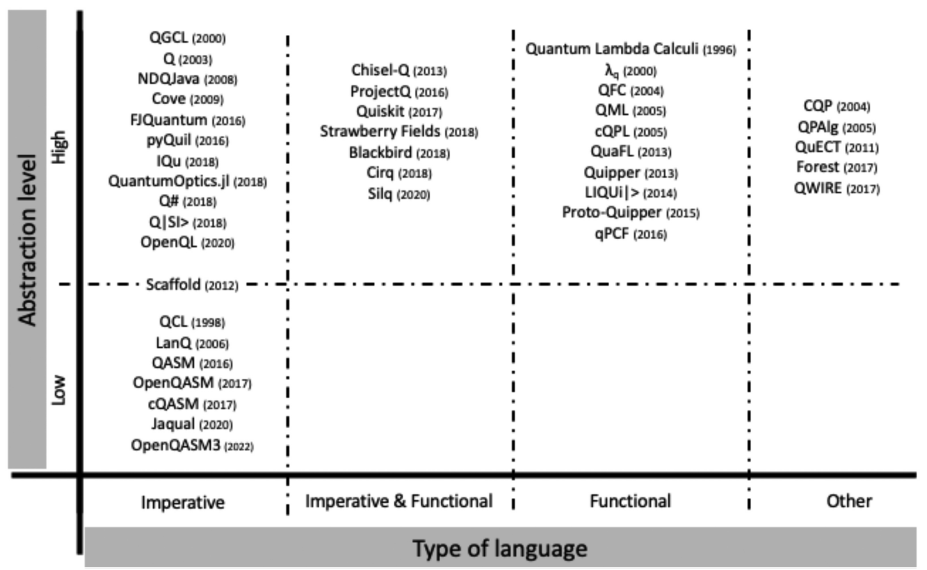
\includegraphics[width=0.9\linewidth]{languages/Quantum-Programming-Landscape.png}
    \caption{Übersicht über Quanten-Programmiersprachen nach Abstraktionsebenen und Programmierparadigmen \autocite[][]{serrano_quantum_2023}.}
    \label{fig:quantum-landscape}
\end{figure}

\autoref{fig:quantum-landscape} zeigt eine Übersicht über Programmiersprachen nach Abstraktionsebene und Programmierparadigmen (\enquote{Type of language}). Zu beachten ist, dass es bislang keine einheitlich standardisierte Klassifikation von Quantenprogrammiersprachen gibt und diese je nach Quellen variiert. Während \citeauthor{garhwal_quantum_2021} Q\# als eine hybride Programmiersprache hervorgehoben haben, ordnen \citeauthor{serrano_quantum_2023} sie dem imperativen Paradigma zu. 
Unterschiedliche Autoren setzen dabei teils unterschiedliche Schwerpunkte, was zu divergierenden Einordnungen führen kann. Angesichts der uneinheitlichen Einordnungen in der Literatur erscheint die Erarbeitung eines standardisierten Klassifikationsschemas als eine relevante Aufgabe für zukünftige Forschungsarbeiten.

\subsubsection*{Hardwarebindung}

Die Hardwarebindung einer Quanten-Pro\-gram\-mier\-sprache oder eines Frameworks beschreibt, inwieweit sie an eine bestimmte Quanten\-hardware-Plattform gebunden ist. Man unterscheidet zwischen Hardware-spezifisch und Hardware-unabhängig.

\textit{Hardware-spezifische} Frameworks sind für die Optimierung und Ausführung auf einer bestimmten Architektur konzipiert und optimiert. Sie nutzen die spezifischen Eigenschaften und Einschränkungen der Hardware zur Maximierung der Leistung. Beispiele hierfür sind Cirq \footnote{Cirq \url{https://quantumai.google/cirq}}, optimiert für Google Sycamore Hardware oder PyQuil, optimiert für Rigetti´s Quantum Cloud Service\footnote{Rigetti \url{https://www.rigetti.com/what-we-build}}. 

\textit{Hardware-unabhängige} Sprachen und Frameworks sind so konzipiert, dass sie auf einer Vielzahl von Hardware-Plattformen ausgeführt werden können, oft durch die Verwendung von Zwischenrepräsentationen wie OpenQASM. Sie bieten eine große Flexibilität und Portabilität. Zu ihnen gehören unter anderem Qiskit von IBM sowie das Braket SDK von Amazon \autocite{ferreiraExploratoryStudyUsage2025}.

\subsubsection*{Quantenmodell}

Das Quantenmodell beschreibt die dem Quantencomputer zugrunde liegenden physikalischen Prinzipien und Berechnungsmodelle. Hierfür werden Programmiersprachen den Modellen aus \autoref{programming-models} zugeordnet.

Das \textit{Gate-basierte} Modell ist das dominanteste und am weitesten verbreitete Modell, bei dem Quantenalgorithmen durch Schaltkreise aus Quantengattern auf Qubits dargestellt werden. Ein Großteil der aktuellen Quantencomputer und Frameworks basiert auf diesem Modell. Beispiele für Sprachen und Frameworks sind die bereits erwähnten Q\#, Cirq oder OpenQASM. \autocite{ferreiraExploratoryStudyUsage2025}

Das \textit{messungsbasierte} Paradigma (MBQC) führt Berechnungen durch eine Sequenz von Einzel-Qubit-Messungen auf einem vorbereiteten, hochgradig verschränkten Anfangs-Cluster-Zustand durch. Die Wahl der Messbasis für jedes Qubit hängt hierbei von den Ergebnissen früherer Messungen ab. Bisher gibt es wenige produktive Frameworks. Ein prominentes Beispiel ist der One-Way Quantum Computer. One-way (Einweg) ergibt sich daraus, dass jede Messung den Zustand eines Qubits zerstört und die Ressource verbraucht. \citeauthor{briegelMeasurementbasedQuantumComputation2009} bewiesen, dass mithilfe eines zweidimensionalen Cluster-Zustands beliebige Quantenalgorithmen realisiert werden können, wodurch dieses Modell formal als äquivalent zum Schaltkreis-Modell zu sehen ist. \autocite{briegelMeasurementbasedQuantumComputation2009}

Das \textit{adiabatische} Paradigma nutzt Annealing zur Lösung komplexer Optimierungs- und Sampling-Probleme. Annealing übertrifft das Gate-Modell bei Optimierungsproblemen, da es den erheblichen Vorverarbeitungsaufwand vermeidet, der mit Gate-basierten Ansätzen verbunden ist. Darüber hinaus ist es deutlich toleranter gegenüber Fehlern und Rauschen sowie auf die Größe von Unternehmensproblemen skalierbar. \autocite{albash_adiabatic_2018} Das bekannteste Beispiel ist das D-Wave\footnote{D-Wave \url{https://www.dwavequantum.com/solutions-and-products/ocean/}} Ocean SDK, das speziell für adiabatische Quantencomputer entwickelt wurde.

\begin{table}[ht!]
\centering
\footnotesize
\begin{tabularx}{\textwidth}{|l|p{2cm}|l|l|l|X|}
\hline
\textbf{Jahr} & 
\textbf{Sprache / Framework} & 
\textbf{Abstraktionslevel} & 
\textbf{Paradigma} & 
\textbf{Quantenmodell} & 
\textbf{Hostsprache} \\
\hline
2022 & OpenQASM3 & Low-Level & Imperativ & Gate-basiert & Quantum Assembly \\
\hline
2020 & Braket SDK & High-Level & Hybrid & Gate-basiert & Python \\
\hline
2020 & D-Wave Ocean & High-Level & Hybrid & Adiabatisch & Python \\
\hline
2020 & Silq & High-Level & Hybrid & Gate-basiert & Eigenständig \\
\hline
2020 & OpenQL & High-Level & Hybrid & Gate-basiert & Python, C++ \\
\hline
2018 & Cirq & High-Level & Hybrid & Gate-basiert & Python \\
\hline
2018 & Q\# (Microsoft QDK) & High-Level & Hybrid & Gate-basiert & C\# \\
\hline
2018 & Strawberry Fields & High-Level & Hybrid & Kontinuierlich-variabel & Python \\
\hline
2017 & Qiskit & High-Level & Hybrid & Gate-basiert & Python \\
\hline
2017 & OpenQASM & Low-Level & Imperativ &  Gate-basiert & Quantum Assembly \\
\hline
2016 & pyQuil & High-Level & Imperativ &  Gate-basiert & Python \\
\hline
2013 & Quipper & High-Level & Funktional & Gate-basiert & Haskell \\
\hline
2012 & Scaffold & Low-Level & Imperativ &  Gate-basiert & C / C++ \\
\hline
2006 & LanQ & Low-Level & Imperativ & Gate-basiert & C, Java \\
\hline
2005 & QML & High-Level & Funktional & Gate-basiert & Haskell \\
\hline
2003 & Q & High-Level & Imperativ & Gate-basiert & C++ \\
\hline
2000 & qGCL & High-Level & Imperativ &  Gate-basiert & C \\
\hline
1998 & QCL & Low-Level & Imperativ & Gate-basiert & C \\
\hline
1996 & Quantum Lambda Calculi (theoretisches Konzept) & High-Level & Funktional & Gate-basiert & Lambda Calculus \\
\hline
\end{tabularx}
\caption{Erweiterter Vergleich von Quantum-Programmiersprachen und Frameworks}
\label{tab:quantum_languages_full}
\end{table}

In dieser Arbeit werden unter dem Begriff \enquote{Quanten-Programmiersprachen und -Frameworks} sowohl formale, eigenständige Programmiersprachen als auch softwareseitige Entwicklungsumgebungen und Bibliotheken zusammengefasst, die die Programmierung, Ausführung und Analyse von Quantenalgorithmen ermöglichen. Obwohl sich diese Systeme in Aufbau und Fokus teilweise unterscheiden, verfolgen sie das gemeinsame Ziel der Bildung einer Schnittstelle zwischen Quantenalgorithmen und deren Ausführung auf Quantenhardware oder Simulationen. \autoref{tab:quantum_languages_full} fasst die Klassifizierungen beispielhafter Quanten-Programmiersprachen und Frameworks zusammen. Die Einordnung beruht hierbei auf verschiedenen Arbeiten von \autocite{singhSurveyAvailableTools2024a}, \autocite{ferreiraExploratoryStudyUsage2025}, \autocite{garhwal_quantum_2021}, \autocite{serranoQuantumSoftwareComponents2023a} und eigener Einschätzung.

\subsection{Qiskit im Detail}
\label{sec:qiskit-details}

Qiskit ist ein Python-basiertes Open-Source-Softwareentwicklungskit (SDK) von IBM. Es bietet ein umfassendes Ökosystem an Werkzeugen und Plugins zur Erstellung und Bearbeitung von Quantenprogrammen. Diese Programme lassen sich sowohl in der IBM Quantum Experience als auch auf weiteren IBM-unabhängigen Backends ausführen. \autocite{singhSurveyAvailableTools2024a} Darüber hinaus können sie auch lokal simuliert werden, wie das Praxisbeispiel (\autoref{sec:practical-example}) zeigt. 

Qiskit hat sich seit seiner Einführung im Jahr 2017 als ein zentrales Werkzeug in der Quanteninformatik etabliert. Mit über sechs Millionen Installationen und einer monatlichen Installationsrate von 300.000 ist Qiskit die meistgenutzte Software für Quantencomputing. Das Ökosystem wird nicht nur von IBM gepflegt, sondern mittlerweile von einer großen Gemeinschaft aus über 500 Mitwirkenden, die zur Entwicklung von über 300 Python-Paketen beigetragen haben. \autocite{javadi-abhariQuantumComputingQiskit2024a}

\autoref{fig:qiskit-architektur} zeigt die schematische Darstellung der Qiskit-Architektur. Qiskit unterstützt sowohl abstrakte als auch konkrete Repräsentationen von Quantenalgorithmen. Als High-Level-Programmiersprache werden Algorithmen auf hoher Abstraktionsebene als logische Operationen modelliert. Im Zentrum von Qiskit stehen Quantenschaltkreise (Quantum Circuits), um die sich Optimierungs- und Übersetzungswerkzeuge gruppieren. \autocite{javadi-abhariQuantumComputingQiskit2024a}

\begin{figure}[ht!]
    \centering
    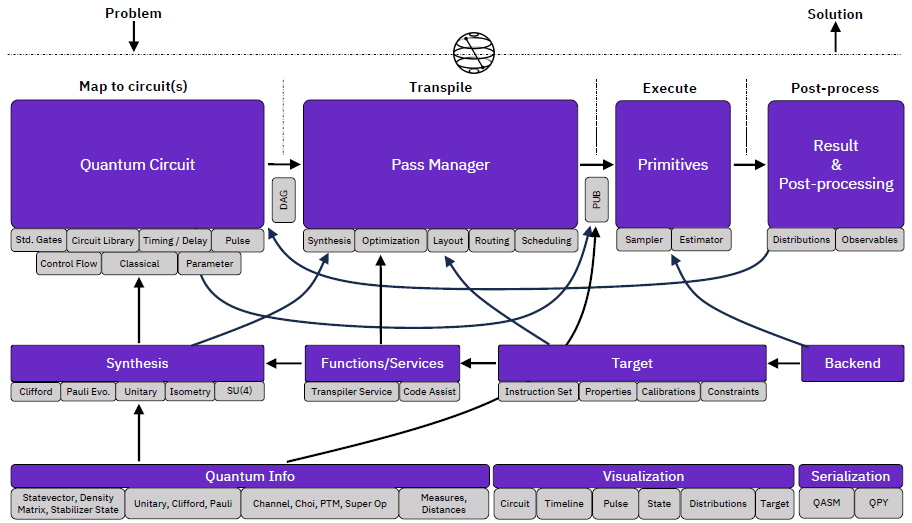
\includegraphics[width=1\linewidth]{languages/Qiskit-Architektur.png}
    \caption{Qiskit-Architektur \autocite{javadi-abhariQuantumComputingQiskit2024a}}
    \label{fig:qiskit-architektur}
\end{figure}

Ein Pass Manager (Transpiler) wendet Transformationen auf den Schaltkreis an, um ihn an das Gate-Set und die Topologie der Zielhardware anzupassen. Dies ermöglicht die Ausführung auf verschiedenen Quantenprozessoren. Der Transpiler folgt dabei einem mehrstufigen Kompilationsschema, bestehend aus der Layout-Auswahl, dem Routing, der Optimierung und der Dekomposition. In der Layout-Auswahl werden logische Qubits zu physischen Qubits zugewiesen und das Routing fügt SWAP-Gates hinzu. In der Optimierung wird die Anzahl von Gattern und die Schaltungstiefe reduziert und die Dekomposition zerlegt komplexe Operationen in elementare Gates des nativen Gate-Sets der Zielhardware. \autocite{javadi-abhariQuantumComputingQiskit2024a}

Die Zwischensprache OpenQASM dient als Brücke und erlaubt die serielle und strukturierte Repräsentation von Schaltungen. \autocite{crossOpenQuantumAssembly2017a}

Die aufbereiteten Schaltkreise führen die Primitives dann auf Simulatoren oder realen Quantenprozessoren aus. Der Sampler führt einen Schaltkreis aus und liefert die resultierenden Bitstring-Wahrscheinlichkeiten zurück, während der Estimator Erwartungswerte von Observables schätzt.

Qiskit ist modular aufgebaut und folgt einer mehrschichtigen Architektur mit vier Komponenten. Dies ermöglicht es, Quantenprogramme zunächst abstrakt zu formulieren und sie dann für die konkrete Hardware zu optimieren. \autocite{javadi-abhariQuantumComputingQiskit2024a}
\\

\paragraph{1) Terra}
Terra bildet das Fundament des Frameworks und stellt die grundlegenden Datentypen und Werkzeuge bereit, um Quanten-Schaltkreise zu erstellen, zu manipulieren und zwischen Hardware und Software zu vermitteln. Die zentrale Abstraktion ist der in \autoref{fig:qiskit-architektur} dargestellte Quantum Circuit, in dem Gatter, Messungen und Barrieren als sequenzielle Operationen auf Qubits modelliert werden. Darüber hinaus enthält Terra die Implementierung des Transpilers zur Optimierung der Schaltkreise und die Schnittstellen zu Simulatoren und Cloud-QPUs. \autocite{javadi-abhariQuantumComputingQiskit2024a}
\\

\paragraph{2) Aer}
Aer bietet schnelle Simulationen quantenmechanischer Zustände, wie Zustands\-vektor\mbox{-}, Dichtematrix- und Stabilisator-Simulationen, und unterstützt die Modellierung realistischer Rauschprozesse. Die Integration realistischer Rauschmodelle (Noise Models) ermöglicht die Simulation und Optimierung auf echter Hardware. Diese ist essenziell für die Entwicklung von Algorithmen auf NISQ-Geräten. \autocite{javadi-abhariQuantumComputingQiskit2024a}
\\

\paragraph{3) Ignis und Aqua}
Ignis und Aqua waren ursprünglich zwei weitere Komponenten, die mittlerweile in verschiedene separate Module ausgelagert wurden. Ignis enthält Werkzeuge zur Charakterisierung von Hardwarefehlern sowie Fehlermessungs- und -minderungstechniken \footnote{IBM Qiskit \url{https://www.ibm.com/quantum/qiskit/history}}. Aqua konzentriert sich auf die Anwendung von Qiskit auf spezifische Anwendungsfälle. Die Komponente enthält eine Sammlung von Quantenalgorithmen. Dazu gehören Algorithmen für Quantenchemie, Finanzmathematik oder maschinelles Lernen, die Nutzern die Implementierung von Quantenalgorithmen ermöglichen, ohne tief mit den Details der Schaltkreisimplementierung vertraut sein zu müssen. \autocite{javadi-abhariQuantumComputingQiskit2024a}

\section{Quantum Software Engineering}

Das Quantum Software Engineering (QSE) ist ein aufkommendes Teilgebiet der Softwaretechnik, das sich mit der Entwicklung, Integration und Wartung quantenbasierter Softwaresysteme befasst. Im Gegensatz zur klassischen Softwareentwicklung bringt QSE neue Anforderungen mit sich – etwa die Integration probabilistischer Ausführung, hardwareabhängiger Toolchains und hybrider Workflows. \autocite{zhao_quantum-based_2025} Dieses Kapitel beleuchtet zentrale Aspekte der QSE, vom zugrundeliegenden Software-Stack über den Einsatz von Simulatoren und den Zugang zu realer Quantenhardware über Cloud-Plattformen bis hin zur Integration quantenbasierter Anwendungen in moderne Softwareentwicklungsprozesse.

\subsection{Quantum Software Stack}
\label{sec:quantum-software-stack}

Das Quantum Software Engineering benötigt einen mehrschichtigen Software-Stack, mit dem abstrakte Quantenalgorithmen auf Quantenhardware übertragen und ausgeführt werden können. Eine mögliche Strukturierung eines solchen Software-Stacks ist in \autoref{fig:quantum-software-stack} abgebildet und setzt sich aus den drei Ebenen \emph{Nutzer (User Layer)}, \emph{Plattform (Platform Layer)} und \emph{Hardware (Hardware Layer)} zusammen. Jede dieser Schichten übernimmt spezifische Aufgaben innerhalb des Gesamtsystems und abstrahiert die Komplexität der darunterliegenden Ebenen.
\\

\begin{figure}[ht!]
\centering
\begin{tikzpicture}[
  layerbox/.style={
    draw,
    minimum width=6cm,
    minimum height=0.8cm,
    text centered
  }
]

\node[layerbox] (l1) at (0,  0) {Programmiersprachen};
\node[layerbox] (l2) at (0, -1) {SDKs und Frameworks};
\node[layerbox] (l3) at (0, -2) {Quantenalgorithmen};
\node[layerbox] (l4) at (0, -3) {Quantenanwendungen};

\node[layerbox] (l5) at (0, -4.5) {Simulation};
\node[layerbox] (l6) at (0, -5.5) {Kompilierung};
\node[layerbox] (l7) at (0, -6.5) {Fehlerkorrektur};

\node[layerbox] (l8) at (0, -8) {Kontrollsysteme};
\node[layerbox] (l9) at (0, -9) {Quantum Processing Unit (QPU)};

\draw[decorate, decoration={brace, amplitude=6pt, mirror}, very thick]
  ($(l1.north west) + (-0.2,0.1)$) -- ($(l4.south west) + (-0.2,-0.1)$)
  node[midway, xshift=-0.4cm, anchor=east, font=\normalsize\bfseries] {Nutzer};

\draw[decorate, decoration={brace, amplitude=6pt, mirror}, very thick]
  ($(l5.north west) + (-0.2,0.1)$) -- ($(l7.south west) + (-0.2,-0.1)$)
  node[midway, xshift=-0.4cm, anchor=east, font=\normalsize\bfseries] {\textbf{Plattform}};

\draw[decorate, decoration={brace, amplitude=6pt, mirror}, very thick]
  ($(l8.north west) + (-0.2,0.1)$) -- ($(l9.south west) + (-0.2,-0.1)$)
  node[midway, xshift=-0.4cm, anchor=east, font=\normalsize\bfseries] {\textbf{Hardware}};

\end{tikzpicture}
\caption{Struktur eines Quantum Software-Stacks \autocite{ryan_understanding_2024}}
\label{fig:quantum-software-stack}
\end{figure}

\paragraph{Nutzer-Schicht}  
In der obersten Schicht werden Problemstellungen mittels Quantenalgorithmen (\autoref{basic_algorithms} \textbf{TODO: Ref basic-algorithms}) in konkreten Anwendungscode übertragen. Sie umfasst Werkzeuge und Bibliotheken, mit denen Entwickler Quantenalgorithmen und -anwendungen implementieren und für die Ausführung auf Quantenhardware vorbereiten können. Dazu gehören vor allem die in \autoref{sec:programming-languages} näher erläuterten Programmiersprachen und Entwicklungswerkzeuge (SDKs und Frameworks) wie Qiskit, Cirq oder Q\#.
\\

\paragraph{Plattform-Schicht}  
Die Plattformschicht ist für die Kompilierung und Optimierung von Quantenprogrammen zuständig. Dies umfasst Compiler wie TKET oder den Qiskit Transpiler, die den Programmcode in Quantenhardware-kompatible Befehle übersetzen. Dazu zählen z.B. Gate-Dekomposition, Qubit-Zuordnung und Optimierung hinsichtlich Laufzeit und Fehlerresistenz. Auch dedizierte Software zur Fehlerkorrektur wie Riverlane kann dieser Schicht zugeordnet werden. Darüber hinaus enthält die Plattformschicht Simulatoren und Emulatoren -- Software, die echte Quantenhardware nachbildet und so ein einfacheres Testen, Debuggen und Optimieren von Quantenanwendungen ermöglicht.
\\

\paragraph{Hardware-Schicht}  
Am unteren Ende des Software-Stacks befindet sich die eigentliche Quantenhardware (Quantum Processing Unit) sowie Software für deren Verwaltung und Überwachung. Kontrollsysteme wie Quantum Machines OPX+ ermöglichen beispielsweise die Kalibrierung, Pulsgenerierung und qubitgenaue Steuerung der Hardware. Außerdem umfasst die Hardwareschicht weitere Fehlerkorrekturmechanismen.
\\

Jede Schicht im Software-Stack abstrahiert technische Details der darunterliegenden Ebene und trägt zur strukturierten Entwicklung, Optimierung und Ausführung von Quantenprogrammen bei. \autocite{shehata_building_2025} \autocite{ryan_understanding_2024}

\subsection{Simulatoren}
\label{sec:simulators}

Simulatoren ermöglichen als Teil der Plattformschicht des Quantum Software-Stacks die funktionale Ausführung von Quantenalgorithmen auf klassischer Hardware, ohne dass eine physikalische Quantenmaschine benötigt wird.

Simulationen von Quantencomputern lassen sich in drei grundlegende Kategorien einteilen:
\begin{itemize}
\item \textbf{Geräteebene-Simulationen} bilden die physikalischen Eigenschaften und Materialien einzelner Qubits ab und sind mit Hardware-nahen Simulationen klassischer Systeme vergleichbar.
\item \textbf{Gatterebene-Simulationen} modellieren die Ausführung einzelner Quanten-Gates auf bestimmten Qubit-Zuordnungen und fokussieren sich auf die Mikroarchitektur.
\item \textbf{Algorithmusebene-Simulationen} abstrahieren diese physikalischen Details und bilden stattdessen das Verhalten kompletter Quantenalgorithmen und Schaltkreise nach.
\end{itemize}

Im Kontext der Entwicklung von Quantensoftware ist vor allem die Simulation auf algorithmischer Ebene relevant. Hierbei werden vollständige Quantenprogramme in Form von Schaltkreisen simuliert, sodass Entwickler deren Verhalten analysieren, testen und optimieren können. Im Vordergrund steht dabei die logische Korrektheit und Funktionalität des Programms als Ganzes. Diese Form der Simulation ist ein essenzieller Bestandteil der Entwicklungswerkzeuge in modernen SDKs wie Qiskit oder Cirq.

Allerdings unterliegt diese Art der Simulation fundamentalen Einschränkungen: Da der Speicher- und Rechenaufwand exponentiell mit der Anzahl der simulierten Qubits wächst, ist ihre Nutzung auf Programme mit einer vergleichsweise kleinen Qubitanzahl beschränkt. Für komplexere, realitätsnahe Algorithmen und Anwendungen reicht die Simulation daher oft nicht aus -- in solchen Fällen ist der Zugang zu echter Quantenhardware erforderlich. \autocite{cicero_simulation_2025}

\subsection{Quantum Cloud Computing}
\label{sec:quantum-cloud-computing}

Da Quantenhardware in der Anschaffung teuer und im Betrieb hochkomplex ist, stellt das Quantum Cloud Computing (QCC) eine zentrale Möglichkeit dar, um Endnutzern dennoch einen praktischen Zugang zu physikalischer Quantenhardware zu ermöglichen. Über Cloud-Plattformen erhalten sie Zugriff auf Ressourcen, Jobmanagement und Fehlermitigation mittels abstrahierter Schnittstellen in einer skalierbaren Umgebung.

Ein zentraler Vorteil Cloud-basierter Quantenplattformen liegt in ihrer Flexibilität: Nutzer können ihre Rechenkapazitäten bedarfsgerecht skalieren, was die Bearbeitung unterschiedlich komplexer Probleme effizienter gestaltet. Außerdem ermöglichen sie das einfache Entwickeln und Testen von Quantenalgorithmen in simulierten Umgebungen, bevor diese auf echter Hardware ausgeführt werden. Dies reduziert die Einstiegshürden, da keine spezialisierte Infrastruktur oder tiefgreifende Hardwarekenntnisse notwendig sind. Da alle Nutzer auf dieselbe Plattform zugreifen, werden darüber hinaus globale Kollaboration und standardisierte Entwicklungsumgebungen begünstigt.

Zu den wichtigsten Anbietern von Quantum Cloud Plattformen zählen aktuell IBM, Amazon und Google. Ihre Plattformen IBM Quantum\footnote{IBM Quantum \url{https://quantum.ibm.com/}}, Amazon Braket\footnote{Amazon Braket \url{https://aws.amazon.com/braket/}} und Google Quantum AI\footnote{Google Quantum AI \url{https://quantumai.google/cirq/google/concepts}} sind in \autoref{tab:quantum-cloud-platforms} gegenübergestellt \autocite{golec_quantum_2024}.

\begin{table}[ht!]
\centering
\begin{tabular}{|p{2.5cm}|p{4.8cm}|p{4cm}|}
\hline
\textbf{Plattform} & \textbf{Hardware} & \textbf{Unterstützte Sprachen / SDKs} \\
\hline
IBM Quantum & Falcon, Eagle (Supraleitende Qubits) & Qiskit \\
\hline
Amazon Braket & IonQ (Ionenfallen), Rigetti (supraleitend), OQC (Photonik) & Braket SDK, PennyLane, Qiskit \\
\hline
Google Quantum AI & Sycamore (supraleitend) & Cirq \\
\hline
\end{tabular}
\caption{Vergleich führender Quantum Cloud Plattformen}
\label{tab:quantum-cloud-platforms}
\end{table}

Alle drei Plattformen bieten Cloud-basierten Zugang zu Quantenprozessoren im Pay-as-you-go-Modell, wodurch Nutzer ohne hohe Einstiegskosten reale Quantenhardware nutzen können. Dabei unterstützen alle Anbieter hybride Workflows, bei denen klassische und quantenbasierte Berechnungen kombiniert werden. Angesichts der Fehleranfälligkeit heutiger Quantenhardware integrieren alle Plattformen Mechanismen zur Fehlerminderung. Zudem sind alle Plattformen gut in ihre jeweiligen Cloud-Ökosysteme integriert (IBM Cloud, AWS, Google Cloud), um Nutzern eine nahtlose Entwicklung und Verwaltung quantenbasierter Anwendungen zu ermöglichen.

Die drei Plattformen unterscheiden sich vor allem in der Hardwareverfügbarkeit, Softwarearchitektur und ihrem Ausführungsmodell. IBM Quantum bietet exklusiv Zugang zu eigenen supraleitenden Quantenprozessoren, darunter fortschrittliche Geräte wie den 127-Qubit-Eagle. Amazon Braket hingegen fungiert als Meta-Plattform und stellt über eine einheitliche Schnittstelle Zugang zu verschiedenartigen QPUs bereit – z.B. Ionenfallen (IonQ) und supraleitende Systeme (Rigetti, OQC). Google Quantum AI verwendet ausschließlich eigene supraleitende Chips (z.B. Sycamore), die jedoch nur ausgewählten Partnern zugänglich sind. Damit bieten IBM und AWS aktuell breiteren öffentlichen Hardwarezugang, während Google auf forschungsorientierte Hardwareentwicklung mit begrenztem Zugriff setzt.

Auch auf Softwareebene gibt es Unterschiede: IBM unterstützt mit Qiskit ein umfassendes Open-Source SDK. Braket erlaubt mehr Flexibilität, indem es neben dem eigenen SDK auch Drittanbieter-Frameworks wie PennyLane unterstützt. Google verwendet Cirq – ein eher Low-Level-orientiertes SDK, das präzise Kontrolle über qubit-spezifische Details ermöglicht, insbesondere im Kontext von Machine Learning mit TensorFlow Quantum. Bei den Ausführungsmodellen bietet IBM mit Qiskit Runtime ein latenzarmes Session-Modell inklusive dynamischer Schaltungen, während Braket hybride Jobs in AWS-Containern orchestriert. Google hingegen ermöglicht primär Batch-Ausführungen über das Quantum Engine API – ohne öffentliche Hybrid-Job-Funktionalität. \autocite{googleGoogleQuantumComputing2025} \autocite{mittalQiskitRuntimeCloudNative2022} \autocite{amazonwebservicesAmazonBraketFeatures2025}

Darüber hinaus gibt es weitere Plattformen wie etwa \textit{Strangeworks}, \textit{Xanadu}, \textit{Quantinuum}, \textit{IonQ} (auch über Azure Quantum) und \textit{Microsoft Azure Quantum}. Diese bieten entweder eigene Hardwaretechnologien (wie photonische QPUs bei Xanadu oder trapped-ion Systeme bei Quantinuum) oder bündeln übergreifende Multi-Backend-Zugänge mit einheitlicher API. Microsoft ermöglicht zudem tiefe Integration in klassische Azure-Dienste, während Strangeworks auf eine benutzerfreundliche Multi-Vendor-Umgebung setzt.

\subsection{Integration in moderne Entwicklungsprozesse}
\label{sec:integration-devops}

Mit Fortschritten im Quantum Computing wächst auch die Bedeutung moderner DevOps-Methoden, wie sie aus der klassischen Softwaretechnik bekannt sind. Dazu zählen insbesondere die kontinuierliche Integration und Bereitstellung (CI/CD) sowie das automatisierte Testen. Die Vielfalt an Hardwarearchitekturen und die fehlende Standardisierung, beispielsweise die Nutzung von proprietären, plattformspezifischen Programmiersprachen und Werkzeugen, stellen dabei besondere Herausforderungen dar.

Ein aktueller Forschungsansatz ist das Framework QCRAFT, mit dem klassische CI/CD-Prinzipien auf das Quantum Computing übertragen werden können. Es nutzt containerisierte Umgebungen, um Plattformkonsistenz zu gewährleisten, und bindet Werkzeuge wie GitHub Actions in den Entwicklungsprozess ein. Wie in \autoref{fig:qcraft} abgebildet, ist eine zentrale Funktion dabei die automatische Übersetzung von Quantenprogrammen in plattformspezifische Code-Formate wie Qiskit oder Amazon Braket SDK mithilfe des Q-Trans Service. Dadurch lassen sich Quantenanwendungen ohne manuelle Anpassung zwischen Anbietern wie IBM und AWS migrieren, was einen wichtigen Schritt hin zur plattformübergreifenden Interoperabilität und Wiederverwendbarkeit darstellt.

\begin{figure}[ht!]
  \centering
  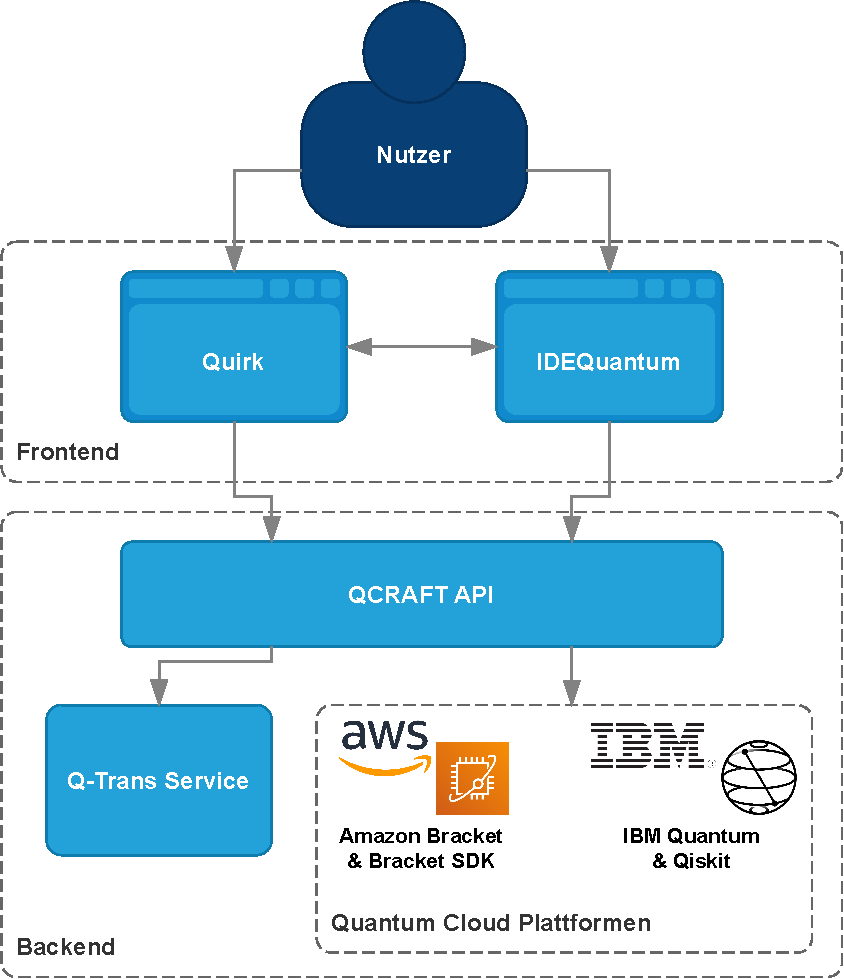
\includegraphics[width=1\textwidth]{qcraft-architecture.pdf}
  \caption{Vereinfachte Architektur des QCRAFT Developer Interface \autocite{romero-alvarez_qcraft_2025}}
  \label{fig:qcraft}
\end{figure}

Durch visuelle Werkzeuge wie Quirk\footnote{Quirk \url{https://algassert.com/quirk}} kann darüber hinaus der Zugang zur Quantenentwicklung vereinfacht werden: Entwickler können Schaltkreise per Drag-and-Drop erstellen und direkt als Services ausliefern. Solche integrierten Entwicklungsumgebungen, die CI/CD, Übersetzung, Deployment und Ausführung kombinieren, tragen wesentlich zur Professionalisierung der quantenbasierten Softwareentwicklung bei und schaffen die Grundlage für skalierbare, wartbare und automatisierbare Prozesse. \autocite{romero-alvarez_qcraft_2025}

\section{Praxisbeispiel: Grover-Suche mit Qiskit}
\label{sec:practical-example}

Abschließend soll anhand eines Beispiels die praktische Umsetzung einer Quantenanwendung veranschaulicht werden. Konkret wird der Grover-Algorithmus zur Lösung eines unstrukturierten Suchproblems implementiert. Der Algorithmus zielt darauf ab, in einem Zustandsraum mit $2^n$ Einträgen einen bestimmten, zuvor markierten Zustand mit signifikant weniger Abfragen zu identifizieren, als dies klassisch möglich wäre.

Die Implementierung erfolgt mit Qiskit auf Grundlage eines Gate-basierten Quantenmodells, wobei zunächst einfache Systeme mit zwei und drei Qubits betrachtet werden. Dabei werden sowohl die theoretischen Grundlagen des Algorithmus als auch dessen Umsetzung in einer realen Quantenentwicklungsumgebung erläutert. Das Beispiel richtet sich insbesondere an Einsteiger und soll die Brücke zwischen abstrakter Theorie und praktischer Anwendung schlagen.

\subsection{Überblick über das Praxisbeispiel}

Im Folgenden wird der grundlegende Ablauf des Grover-Algorithmus skizziert, bevor die einzelnen Schritte anschließend in Qiskit praktisch umgesetzt werden. Ausgangspunkt ist jeweils ein Qubit-Register, das durch die Anwendung von Hadamard-Gattern in eine gleichmäßige Superposition aller möglichen Zustände überführt wird. Diese Phase der Initialisierung erzeugt einen quantenmechanischen Zustand, in dem jeder mögliche Eintrag des Suchraums mit gleicher Amplitude repräsentiert ist. Der nächste Schritt besteht in der Anwendung des sogenannten Orakels, das den gesuchten Zustand durch eine Phaseninversion markiert. In der hier realisierten Version wird im Fall von zwei Qubits der Zustand $|11\rangle$ als Zielzustand definiert und durch ein einfaches CZ-Gatter identifiziert. Für die Erweiterung auf drei Qubits wird entsprechend ein mehrfach kontrolliertes Z-Gatter eingesetzt, das gezielt den Zustand $|111\rangle$ anspricht.

Im Anschluss an das Oracle kommt der sogenannte Diffusionsoperator zur Anwendung, der eine Spiegelung aller Amplituden um ihren Mittelwert bewirkt. Ziel dieses Schritts ist es, die Wahrscheinlichkeit des markierten Zustands zu verstärken, während die übrigen Zustände unterdrückt werden. Die Umsetzung erfolgt durch eine festgelegte Folge elementarer Gatter, darunter Hadamard-, X- und kontrollierte NOT-Gatter. Bereits nach einer einzigen Iteration dieses Verfahrens – bei kleinen Registern in der Regel ausreichend – ist der Zielzustand in der quantenmechanischen Wahrscheinlichkeitsverteilung deutlich hervorgehoben.

Die finale Messung der Qubits erfolgt am Ende des Algorithmus. Dabei zeigt sich, dass der zuvor markierte Zustand mit hoher Wahrscheinlichkeit detektiert wird. Die experimentelle Auswertung bestätigt die theoretische Erwartung: Der Grover-Algorithmus führt zu einer gezielten Verstärkung des gewünschten Ergebnisses. Dies wird insbesondere durch die grafische Darstellung der Messhäufigkeiten deutlich, bei der der Zielzustand als klar dominanter Messwert erscheint.

Insgesamt zeigt dieses Beispiel, wie sich ein komplexer quantenmechanischer Algorithmus mit relativ einfachen Mitteln umsetzen lässt. Die Verbindung von Theorie und Praxis wird damit greifbar: Während im Kapitel Quantenalgorithmen \textbf{TODO:REF} die mathematische Grundlage gelegt wird, bietet die hier vorgestellte Implementierung eine konkrete Anwendung und liefert gleichzeitig einen Einstieg in den praktischen Umgang mit modernen Quantenentwicklungstools.

\subsection{Implementierung einer Grover-Suche mit Qiskit}
\label{sec:grover-implementation}

Zur praktischen Umsetzung wird eine lokale Python-Umgebung eingerichtet, in der die Programmbibliothek \texttt{qiskit} installiert wird. Die Verwendung einer virtuellen Umgebung (\texttt{venv}) gewährleistet dabei, dass projektbezogene Abhängigkeiten isoliert bleiben und mit anderen Projekten nicht in Konflikt geraten. Für die interaktive Arbeit mit Quantenalgorithmen kommt das Werkzeug Jupyter Notebook zum Einsatz, was über einen integrierten Webserver verfügt. \autoref{tab:qiskit-anforderungen} zeigt die Systemvoraussetzungen, während \autoref{tab:qiskit-setup} die wesentlichen Installations- und Einrichtungsschritte zusammenfasst.

Um den Grover-Algorithmus praktisch auf einem Quantencomputer umzusetzen, wird eine konkrete Konstruktion der Schaltung benötigt. Der Algorithmus setzt sich dabei aus fünf wesentlichen Komponenten zusammen: 
\begin{enumerate}
    \item  \textbf{Initialisierung:} Vorbereitung aller Qubits im Zustand $\ket{0}$.
    \item \textbf{Superposition:} Erzeugung einer gleichmäßigen Überlagerung aller möglichen Basiszustände durch Anwendung von Hadamard-Gattern
    \item \textbf{Oracle:} Im Oracle wird der gesuchte Zustand, welchen der Grover-Algorithmus identifizieren soll, ausgewählt.
    \item \textbf{Diffusionsoperator:} Der Diffusionsoperator verstärkt durch Interferenz den Zustand des Oracle.
    \item   \textbf{Messung:} Abgeschlossen wird der Algorithmus mit der Messung, um das Ergebnis zu erhalten. 
\end{enumerate}

Diese fünf Schritte können für eine beliebige Anzahl an Qubits angewendet werden. Im Folgenden werden die Komponenten jeweils mathematisch, konzeptionell und praktisch näher ausgeführt. Für den praktischen Teil wird ein Grover-Algorithmus mit Qiskit in Jupyter Notebooks implementiert.

\begin{table}[ht!]
\centering
\begin{tabularx}{\textwidth}{|l|X|}
\hline
\textbf{Komponente} & \textbf{Anforderung} \\
\hline
Betriebssystem & Windows 10 oder 11 (64-Bit) \\
\hline
Python-Version & 3.8 bis 3.11 \\
\hline
Arbeitsspeicher & Mindestens 4 GB (empfohlen: 8 GB oder mehr) \\
\hline
Festplattenspeicher & 1–2 GB freier Speicherplatz \\
\hline
Internetverbindung & Für Installation, Updates und IBM-Zugriff \\
\hline
\end{tabularx}
\caption{Systemanforderungen für die Qiskit-Installation}
\label{tab:qiskit-anforderungen}
\end{table}

\begin{table}[ht!]
\centering
\begin{tabular}{|c|p{4.5cm}|p{6cm}|}
\hline
\textbf{Schritt} & \textbf{Beschreibung} & \textbf{Befehl} \\
\hline
1 & Virtuelle Umgebung erstellen & \protect\mintinline{bash}|python -m venv quantum-env| \\
\hline
2 & Umgebung aktivieren (Windows) & \protect\mintinline{bash}|.\Scripts\activate| \\
\hline
3 & pip-Version prüfen & \protect\mintinline{bash}|pip --version| \\
\hline
4 & Qiskit installieren & \protect\mintinline{bash}|pip install qiskit| \\
\hline
5 & Visualisierungspakete (optional) & \protect\mintinline{bash}|pip install qiskit[visualization]| \\
\hline
6 & IBM Runtime installieren (optional) & \protect\mintinline{bash}|pip install qiskit-ibm-runtime| \\
\hline
7 & Jupyter Notebook installieren & \protect\mintinline{bash}|pip install jupyter| \\
\hline
8 & Jupyter Notebook starten & \protect\mintinline{bash}|jupyter notebook| \\
\hline
\end{tabular}
\caption{Installations- und Einrichtungsschritte für Qiskit}
\label{tab:qiskit-setup}
\end{table}

\subsubsection*{Initialisierung und Superposition}
Der Startzustand aller Qubits ist $\ket{0}$. Um eine gleichverteilte Superposition über alle Basiszustände der Qubits zu erzeugen, muss für jedes der Qubits ein Hadamard-Gate ($H$) angewendet werden. Für die Anzahl $n$ Qubits ist dieser Zusammenhang in \autoref{eq:grover-init} dargestellt. Dieser Zustand bildet die Grundlage für die Amplitudenverstärkung von Grover's Algorithmus. Jede Lösung hat damit zunächst dieselbe Wahrscheinlichkeit. \autocite[257]{nielsen_quantum_2010}

\begin{equation}
\label{eq:grover-init}
|\psi_0\rangle = H^{\otimes n}|0\rangle^{\otimes n} = \frac{1}{\sqrt{2^n}} \sum_{x=0}^{2^n-1} |x\rangle
\end{equation}

Um die Initialisierung praktisch umzusetzen, wird die Python-Bibliothek \textit{QuantumCircuit} benötigt. Anschließend erfolgt die Umsetzung analog zu \autoref{code:groverInit}. Das gewählte Beispiel nutzt zwei Qubits, kann jedoch für die Anzahl $n$ Qubits beliebig erweitert werden.

\begin{listing}[ht!]
  \inputminted{python}{code/grover-init.py}
  \caption{Initialisierung und Superposition des Grover-Algorithmus für 2 Qubits}
  \label{code:groverInit}
\end{listing}

\subsubsection*{Oracle}
Der nächste Schritt in der Implementierung des Grover-Algorithmus ist das sogenannte Oracle. Beim Oracle handelt es sich um eine unitäre Operation $U_f$, welche den gesuchten Zielzustand $\ket{T}$ durch eine Phaseninversion der Qubits kenntlich macht. Das bedeutet konkret, dass der markierte Zielzustand bei Anwendung des Oracles sein Vorzeichen wechselt, während alle anderen Zustände unverändert bleiben. Dieser Zusammenhang wird formal mit \autoref{eq:grover-oracle} beschrieben.

\begin{equation}
\label{eq:grover-oracle}
U_f|x\rangle = \begin{cases}
    -|x\rangle & \text{wenn } x = T \\
    |x\rangle & \text{sonst}
\end{cases}
\end{equation}

\autoref{eq:grover-oracle-ideal} zeigt die formale Beschreibung eines idealen Oracles. Diese Darstellung stammt aus dem Paper \citetitle{roy_deterministic_2022}, wo das Oracle als generalisierte Phasenrotation beschrieben wird. \autocite[2]{roy_deterministic_2022}.

\begin{equation}
\label{eq:grover-oracle-ideal}
S_0(\alpha) = I - (1 - e^{i\alpha})|T\rangle\langle T|
\end{equation}

Für die Standardversion des Grover-Algorithmus wird der Phasenwinkel $\alpha = \pi$ gesetzt, woraus sich die klassische Formel des Grover-Algorithmus (\autoref{eq:grover-formula}) ergibt. Die daraus entstehende Inversion lässt sich als eine Reflexion des Zustandsvektors im sogenannten Hilbertraum interpretieren. 

\begin{equation}
\label{eq:grover-formula}
S_o(\pi) = I - 2|T\rangle\langle T|
\end{equation}

Zur praktischen Umsetzung des Oracles wird das Beispiel aus \autoref{code:groverInit} fortgesetzt. Bei der Implementierung eines Oracles in Qiskit wird häufig das Controlled-Z-Gate (CZ-Gate) genutzt. 

Dieses Gate wirkt standardmäßig nur für den Zustand $\ket{11}$. Um einen anderen Zustand zu markieren, z.B. die anderen 3 möglichen Zustände $\ket{01}$, $\ket{10}$ oder $\ket{00}$, müssen X-Gates (NOT-Gates) eingesetzt werden. Diese transformieren den gewünschten Zielzustand temporär in den Zustand $\ket{11}$. Wenn nach der Transformation zum Zustand $\ket{11}$ das CZ-Gate angewendet wurde, wird das X-Gate erneut ausgeführt, um zur ursprünglichen Codierung des Zustands zurückzukehren.

Nun soll beispielhaft der Zielzustand $\ket{01}$ markiert werden. Dazu ist zunächst das Verständnis der in \autoref{code:grover-oracle-inversion} dargestellten Invertierung von Qubits notwendig.

In Qiskit bedeutet \mintinline{python}{oracle.x(0)}, dass das erste Qubit (Qubit 0) invertiert wird: 0 wird zu 1 und 1 wird zu 0. Analog hierzu invertiert \mintinline{python}{oracle.x(1)} das zweite Qubit (Qubit 1). Dadurch lassen sich gezielt alle Zustände in Zustand $\ket{11}$ umwandeln, auf die dann das CZ-Gate wirken kann.

\begin{listing}[ht!]
  \inputminted{python}{code/grover-oracle-inversion.py}
  \caption{Invertierung der Qubits}
  \label{code:grover-oracle-inversion}
\end{listing}

Um den Zustand $\ket{01}$ zu markieren, wird das erste Qubit (Index 0) mit einem X-Gate invertiert, sodass aus $\ket{0}$ eine $\ket{1}$ wird. Das zweite Qubit (Index 1) bleibt $\ket{1}$. Somit wird aus dem Zustand $\ket{01}$ der Zustand $\ket{11}$. Anschließend wird das CZ-Gate angewandt und das erste Qubit wieder zurückinvertiert, um den Ursprungszustand wiederherzustellen (\autoref{code:grover-oracle-marking}).

\begin{listing}[ht!]
  \inputminted{python}{code/grover-oracle-marking.py}
  \caption{Markierung des Zielzustands $\ket{01}$}
  \label{code:grover-oracle-marking}
\end{listing}

Mit der beschriebenen Vorgehensweise können beliebige Zielzustände (im Fall von zwei Qubits die Zustände $\ket{00}$, $\ket{01}$, $\ket{10}$ und $\ket{11}$) einfach und ohne zusätzliche Hilfs-Qubits realisiert werden. Das funktioniert auch für eine Anzahl $n$ Qubits. \autoref{tab:cz-xgates} zeigt für zwei Qubits, wie man durch die gezielte Anwendung von X-Gates beliebige Zielzustände mit einem CZ-Gate markieren kann. \autocite{roy_deterministic_2022}

\begin{table}[ht!]
\centering
\begin{tabularx}{\textwidth}{|c|X|c|c|}
\hline
\textbf{Zielzustand $|z_1 z_0\rangle$} & \textbf{Beschreibung} & \textbf{Vor dem CZ (X-Gates)} & \textbf{Nach dem CZ (X-Gates)} \\
\hline
$|00\rangle$ & Beide Qubits sind 0 & \texttt{x(0); x(1)} & \texttt{x(0); x(1)} \\
\hline
$|01\rangle$ & Qubit 1 = 0, Qubit 0 = 1 & \texttt{x(0)} & \texttt{x(0)} \\
\hline
$|10\rangle$ & Qubit 1 = 1, Qubit 0 = 0 & \texttt{x(1)} & \texttt{x(1)} \\
\hline
$|11\rangle$ & Beide Qubits sind bereits 1 & – & – \\
\hline
\end{tabularx}
\caption{Markierung beliebiger Zielzustände}
\label{tab:cz-xgates}
\end{table}

\subsubsection*{Diffusionsoperator}

Der Diffusionsoperator, welcher häufig \enquote{Inversion about the mean} genannt wird, verstärkt den im Oracle markierten Zielzustand, indem er alle Amplituden am Mittelwert reflektiert.

\begin{equation}
\label{eq:grover-diffusion}
D = 2|\psi\rangle\langle\psi| - I
\end{equation}

Der Diffusionsoperator ist durch \autoref{eq:grover-diffusion} definiert. Dabei steht der Parameter $|\psi\rangle$ für den gleichverteilten Zustand. Das entspricht aus geometrischer Sicht einer Spiegelung im Hilbertraum. Genau diese Operation ist für die Verstärkung des im Oracle markierten Zielzustands verantwortlich. Nach jeder Grover-Iteration bewirkt sie eine Rotation des Zustandsvektors um einen festen Winkel im Unterraum von markierten und unmarkierten Zuständen. \autocite{nielsen_quantum_2010}

Für zwei Qubits kann der Diffusionsoperator in Qiskit wie in \autoref{code:grover-diffusion} dargestellt umgesetzt werden.

\begin{listing}[ht!]
  \inputminted{python}{code/grover-diffusion.py}
  \caption{Umsetzung des Diffusionsoperators}
  \label{code:grover-diffusion}
\end{listing}

Alternativ ist auch eine Umsetzung mit dem \texttt{GroverOperator} aus der Qiskit-Bibliothek möglich (\autoref{code:grover-diffusion-alternative}).

\begin{listing}[ht!]
  \inputminted{python}{code/grover-diffusion-alternative.py}
  \caption{Alternative Umsetzung des Diffusionsoperators mit dem \texttt{GroverOperator}}
  \label{code:grover-diffusion-alternative}
\end{listing}

\subsubsection*{Messung}

Der abschließende Schritt im Grover-Algorithmus ist die Messung. Diese erfolgt nach mehreren Iterationen von Oracle und Diffusion (typischerweise $\approx \frac{\pi}{4} \sqrt{2^n}$).

\autoref{code:grover-measure} überführt den quantenmechanischen Zustand in einen klassischen Bitstring. Die Wahrscheinlichkeit, bei der Messung den markierten Zustand zu erhalten, ist nun maximal. Bei Nutzung einer Simulation erfolgt diese Messung häufig mehrfach in sogenannten \enquote{shots}, um eine Wahrscheinlichkeitsverteilung zu erhalten. So lässt sich die Dominanz des gesuchten Zustands gegenüber den anderen Zuständen statistisch nachweisen.

\begin{listing}[ht!]
  \inputminted{python}{code/grover-measure.py}
  \caption{Implementierung der Messung}
  \label{code:grover-measure}
\end{listing}
 
Die Konstruktion des Grover-Circuits ist modular und besteht wie beschrieben aus den genannten fünf klar definierten Schritten. Mithilfe von Qiskit lassen sich diese Schritte präzise implementieren, debuggen und simulieren. Das kann sowohl für die theoretische Analyse als auch für praktische Experimente auf realen Quantencomputern verwendet werden. \autocite{ibm_quantum_2025} \autocite{noauthor_grovers_nodate}

\subsection{Visualisierung von Schaltkreis und Ergebnissen}

Ein zentrales Anliegen beim Verständnis und bei der Vermittlung von Quantenalgorithmen ist die Möglichkeit, deren Funktionsweise nicht nur abstrakt-mathematisch, sondern auch visuell nachvollziehen zu können. Das folgende Kapitel widmet sich der Visualisierung des Grover-Algorithmus anhand zweier Implementierungen – einmal mit zwei, einmal mit drei Qubits – unter Verwendung des Qiskit-Frameworks. Sowohl der Aufbau des Quanten-Schaltkreises als auch die Messergebnisse werden grafisch dargestellt und interpretiert.

\subsubsection*{Visualisierung des Quantenschaltkreises}
\label{sec:grover-visualization}

Für beide Varianten des Grover-Algorithmus wird der jeweilige Quanten-Schaltkreis mit der Methode \mintinline{python}{grover_circuit.draw()} visualisiert. Die resultierende Darstellung (\autoref{fig:grover-visualize-circuit}) erlaubt einen direkten Einblick in den logischen Aufbau des Algorithmus, insbesondere in die Abfolge und Wirkung der in \autoref{sec:grover-implementation} beschriebenen verschiedenen quantenmechanischen Operationen.

\begin{figure}
      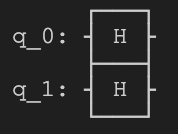
\includegraphics[width=0.25\linewidth]{circuit_superposition.png}
      \caption{Visualisierung des Schaltkreises (Superposition)}
      \label{fig:grover-visualize-circuit}
\end{figure}

\subsubsection*{Visualisierung der Messergebnisse}

Nach Ausführung des Algorithmus auf einem Quantensimulator – konkret dem QASM-Simulator von Qiskit – erfolgt die Analyse der Ergebnisse durch grafische Darstellung der Messausgänge als Histogramm (\autoref{code:grover-visualize-measure}).  

\begin{listing}[ht!]
  \inputminted{python}{code/grover-visualize-measure.py}
  \caption{Implementierung der Visualisierung von Messergebnissen}
  \label{code:grover-visualize-measure}
\end{listing}

In der erzeugten Darstellung (\autoref{fig:visualize-measure}) repräsentiert die Höhe der jeweiligen Balken die Häufigkeit (bzw. Wahrscheinlichkeit) eines bestimmten Bitmusters, das bei der Messung beobachtet wurde.

\begin{figure}
    \centering
    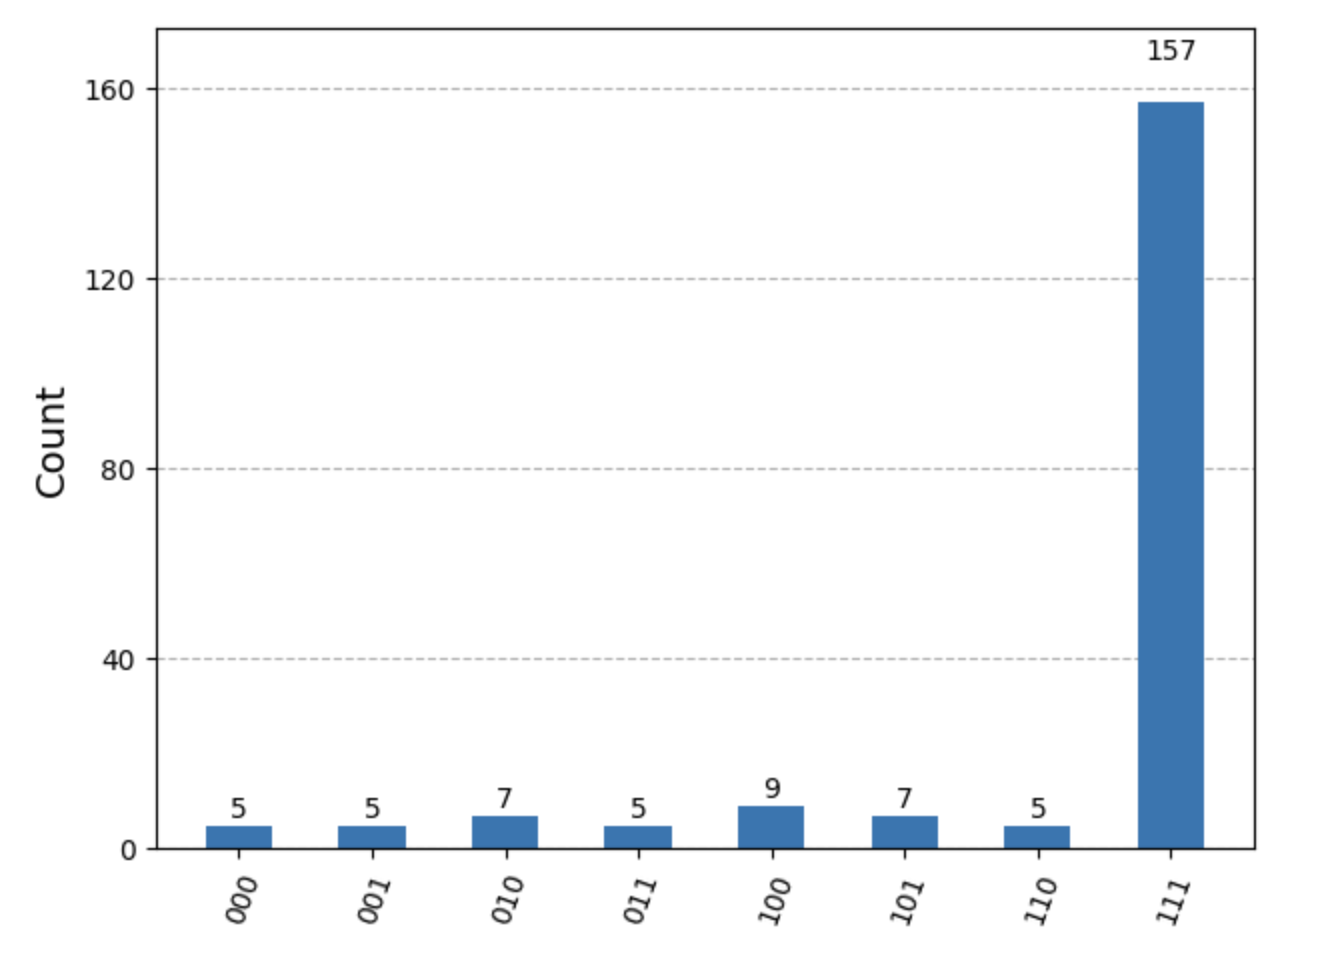
\includegraphics[width=0.75\linewidth]{visualize-measurements.png}
    \caption{Visualisierung der Messergebnisse}
    \label{fig:visualize-measure}
\end{figure}

Im Idealfall – das heißt, bei korrekter Funktionsweise des Orakels und des Grover-Operators – zeigt das Histogramm einen klar dominanten Peak beim Zielzustand.  Die Wahrscheinlichkeiten für alle anderen Zustände bleiben deutlich geringer.  Der gesuchte Zustand hebt sich somit durch quantenmechanische Verstärkung deutlich ab.

\subsection{Testen und Debugging}

Bei der Entwicklung von Quantenalgorithmen spielt die systematische Überprüfung des Codes eine entscheidende Rolle. Quantenprogramme sind nicht nur aufgrund ihrer Komplexität fehleranfällig, sondern verhalten sich auch häufig nicht intuitiv, da viele Zustände nicht direkt beobachtbar sind. Deshalb ist es essenziell, gezielt mit Tests, Zwischenergebnissen und Visualisierungen zu arbeiten, um Fehler zu erkennen und zu beheben. Nachfolgend sind ausgewählte Methoden vorgestellt, mit denen das zuvor mit Qiskit implementierte Quantenprogramm überprüft werden kann.

\subsubsection*{Schrittweise Entwicklung}
Das in \autoref{sec:grover-implementation} beschriebene schrittweise Aufbauen des Grover-Algorithmus ist eine erste Form des \enquote{Testens durch Design}. Einzelne Operatoren und Zustände können nach und nach erzeugt werden, bevor sie in die Gesamtschaltung integriert werden. Durch das schrittweise Ergänzen der Gates kann bereits in frühen Phasen kontrolliert werden, ob jede Transformation wie gewünscht wirkt. Dies entspricht einem iterativen Debugging-Verfahren.

\subsubsection*{Visualisierung als Debugging-Werkzeug}

Wie in \autoref{sec:grover-visualization} gezeigt, kann in Qiskit der Schaltkreis mit geringem Aufwand visualisiert werden. Dies erfüllt nicht nur dokumentarische, sondern auch diagnostische Zwecke. Es kann dadurch überprüft werden, ob etwa das Oracle korrekt umgesetzt oder die Anzahl der Grover-Iterationen richtig gewählt wurde. Fehlende oder falsch platzierte Gates werden so unmittelbar sichtbar. Besonders hilfreich ist dies bei komplexeren Operatorfolgen wie bei Implementierungen mit mehr als zwei Qubits.

\subsubsection*{Ergebnisanalyse durch Histogramme}

Ein weiteres effektives Mittel zur Fehlererkennung ist die statistische Analyse der Messergebnisse (\autoref{sec:grover-visualization}), wie z.B. in \autoref{fig:visualize-measure} dargestellt. Die mit \mintinline{python}{plot_histogram()} erzeugten Verteilungen lassen Rückschlüsse auf das Verhalten des Algorithmus zu. Tritt der erwartete Peak beim Zielzustand nicht auf, kann dies auf einen Fehler im Oracle, in der Grover-Iteration oder in der Initialisierung hinweisen. Wurde beispielsweise ein falsches CZ-Gatter verwendet oder versehentlich eine falsche Qubit-Reihenfolge angesprochen, so verteilt sich die Wahrscheinlichkeitsmasse ungleichmäßig oder falsch.

\subsection{Fazit und Gesamtüberblick}

Das vorliegende Beispiel hat gezeigt, wie sich der Grover-Algorithmus mit Qiskit in einer realitätsnahen Entwicklungsumgebung umsetzen lässt. Beginnend mit der Superposition der Qubits über das markierungsspezifische Oracle bis hin zur Diffusion und abschließenden Messung wurde jeder Bestandteil des Algorithmus in klar abgegrenzten Schritten entwickelt. Die Ergebnisse der finalen Messung illustrieren dabei eindrucksvoll die Effektivität der quantenmechanischen Verstärkung des Zielzustands.

\begin{listing}[ht!]
  \inputminted{python}{code/grover-full.py}
  \caption{Vollständiges Jupyter Notebook für einen Grover-Algorithmus mit zwei Qubits}
  \label{code:grover-full}
\end{listing}

Die vollständige Implementierung inklusive aller Schritte ist in \autoref{code:grover-full} zusammengefasst. Dort ist der gesamte Code zur Ausführung des Algorithmus für zwei Qubits dargestellt – inklusive Initialisierung, Oracle, Diffusionsoperator und Auswertung der Messergebnisse.

Dieses Beispiel unterstreicht das Potenzial moderner Quantum SDKs wie Qiskit für die explorative und forschungsnahe Entwicklung und bietet einen praxisorientierten Einstieg in die Programmierung von Quantenalgorithmen.

\clearpage
\printbibliography
